\documentclass{article}

% ===== Graphics =====
\usepackage{graphicx}
\usepackage{svg}
\graphicspath{{resources/}}
% Colors, table rule color, and caption styling
\usepackage[table]{xcolor}
\definecolor{darkgray}{HTML}{404040}
\arrayrulecolor{darkgray}
\usepackage{caption}
\captionsetup{labelfont={color=darkgray},textfont={color=darkgray}}
\usepackage{array}
\usepackage{tabularx}
\usepackage{threeparttable}
\usepackage{amsmath,amssymb}
\usepackage{tabularx}
\usepackage{dblfloatfix}

\usepackage[colorlinks=true,
linkcolor=blue,    % internal links (sections, equations, etc.)
citecolor=blue,    % citations in the bibliography
urlcolor=blue]     % URLs
{hyperref}





% --- required ---
\usepackage{xcolor}

% --- colors ---
\definecolor{usa_teal}{RGB}{0,255,255}
\definecolor{cn_orange}{RGB}{255,191,0}
\definecolor{eu_purple}{RGB}{255,0,255}
\definecolor{row_grey}{RGB}{220,220,220}


% 2) Make all badges the same size (inner width)
\newlength{\rankbadgewidth}
\setlength{\rankbadgewidth}{1.5em}  % fits 1–100 in bold

\newcommand{\badgebox}[2]{% #1=color, #2=rank text
	{\setlength{\fboxsep}{0.6pt}%
		\colorbox{#1}{\makebox[\rankbadgewidth][c]{\strut\textbf{#2}}}%
	}%
}


% --- EU-27 registry (silent; no text output) ---
\makeatletter
\def\EU@AT{}\def\EU@BE{}\def\EU@BG{}\def\EU@HR{}\def\EU@CY{}\def\EU@CZ{}\def\EU@DK{}\def\EU@EE{}%
\def\EU@FI{}\def\EU@FR{}\def\EU@DE{}\def\EU@GR{}\def\EU@HU{}\def\EU@IE{}\def\EU@IT{}\def\EU@LV{}%
\def\EU@LT{}\def\EU@LU{}\def\EU@MT{}\def\EU@NL{}\def\EU@PL{}\def\EU@PT{}\def\EU@RO{}\def\EU@SK{}%
\def\EU@SI{}\def\EU@ES{}\def\EU@SE{}%
% \IfEU{<ISO>}{<true>}{<false>}
\newcommand{\IfEU}[3]{%
	\edef\ISOtmp{#1}%
	\expandafter\@ifundefined\expandafter{EU@\ISOtmp}{#3}{#2}%
}
\makeatother

% --- choose badge color by ISO-2 (expects UPPERCASE ISO) ---
% Usage: \rankbadge{<rank>}{<ISO2>}
\newcommand{\rankbadge}[2]{%
	\begingroup
	\def\ISO{#2}%
	\def\US{US}\def\CN{CN}%
	\def\badgecol{row_grey}%
	\ifx\ISO\US \def\badgecol{usa_teal}\fi
	\ifx\ISO\CN \def\badgecol{cn_orange}\fi
	\IfEU{\ISO}{\def\badgecol{eu_purple}}{}%

	\def\HK{HK}\def\MO{MO}\def\TW{TW}%
	\ifx\ISO\HK \def\badgecol{cn_orange}\fi
	\ifx\ISO\MO \def\badgecol{cn_orange}\fi
	\ifx\ISO\TW \def\badgecol{cn_orange}\fi
	\makebox[2.4em][c]{\badgebox{\badgecol}{#1}}%
	\endgroup
}

% convenience alias used in the table
\newcommand{\rc}[2]{\rankbadge{#1}{#2}}



% Optional, for nicer rules and spacing
\usepackage{booktabs}



% ===== Colors =====
\usepackage{xcolor}
\definecolor{darkergray}{gray}{0.25}

% ===== Page layout =====
\usepackage[
letterpaper,
top=2.5cm,
bottom=2.5cm,
left=1.5cm,
right=1.5cm,
columnsep=20pt
]{geometry}


% ===== Bibliography with biblatex =====
\usepackage[
backend=biber,
style=numeric,
sorting=none
]{biblatex}
\addbibresource{resources/bibliography.bib} % <-- your .bib file location

\renewcommand*{\bibfont}{\footnotesize}  % Very small font
\setlength{\bibitemsep}{0.25em}         % Tight spacing

% ===== Other styling =====
\usepackage{parskip}    % no indentation, space between paragraphs
\usepackage{titlesec}   % custom section titles
\usepackage{amsmath}
\usepackage{ragged2e}   % for \justifying
\usepackage{microtype}  % better typography
\usepackage{hyperref}   % hyperlinks
\usepackage{float}
\usepackage{paralist}
\usepackage{placeins}
\usepackage{balance}
\usepackage{fancyhdr}
\pagestyle{fancy}
\fancyhf{} % clear all header and footer fields
\fancyhead[R]{\thepage} % page number in top right corner
\renewcommand{\headrulewidth}{0pt}
\renewcommand{\footrulewidth}{0pt} % remove footer line
\pagenumbering{gobble}



% ===== Justification and bad box fixes =====
\AtBeginDocument{\justifying}
\sloppy
\setlength{\RaggedRightRightskip}{0pt plus 0.1\textwidth}

% ===== Section title formatting =====
\titleformat{\section}
{\normalfont\large\bfseries\centering\MakeUppercase}
{\thesection.}{1em}{}
\titleformat{\subsection}
{\normalfont\large\bfseries\centering\MakeUppercase}
{\thesubsection.}{1em}{}

\titlespacing*{\section}{0pt}{3.25ex plus 1ex minus .2ex}{1.5ex plus .2ex}
\titlespacing*{\subsection}{0pt}{3.25ex plus 1ex minus .2ex}{1.5ex plus .2ex}

% ===== Document metadata =====
\title{Mapping National AI Research Authority through Subdisciplinary Differentiation: A Scientometric Study Using OpenAlex (2020–2025)}
\author{Julius Pfundstein \\[1em]
	University of Leipzig \\
	Digital Humanities \\
	julius.pfundstein@studserv.uni-leipzig.de}
\date{Oktober 2025}

\begin{document}

\color{darkergray}


\begin{titlepage}
	
	\vspace*{1cm}
	\centering
	{\LARGE\bfseries Mapping National Artificial Intelligence Research Authority\par}
	\vspace{1em}
	{\LARGE\bfseries A Scientometric Analysis of AI Subdisciplines Using OpenAlex (2020–2025)\par}
	\vspace{3cm}

    {\large
             Julius Pfundstein \\ \vspace{2em}
             Faculty of Mathematics and Computer Science \\ \vspace{2em}
             University of Leipzig \\ \vspace{2em}
             julius.pfundstein@studserv.uni-leipzig.de \par}
    
    % Logo section
    \vspace{3cm}
		\includegraphics[height=3cm, keepaspectratio]{university_of_leipzig_logo.pdf} % Fixed height of 
    
    % Date section
    \vspace{3cm}  % Space between logo and date
    {\large Oktober 2025 \par}
    
    \vfill
    \thispagestyle{empty}
\end{titlepage}

\cleardoublepage
\thispagestyle{empty}

\vspace*{4cm}

\begin{center}
	\Huge\textbf{Acknowledgments}
\end{center}

\vspace{2cm}

\noindent
I would like to express my deepest gratitude to my supervisor,\\
\textbf{Dr. Thomas Efer},\\
for his invaluable guidance, continuous support, and insightful feedback throughout the course of my master’s thesis.

\vspace{1cm}

\noindent
I also wish to sincerely thank the OpenAlex team for generously providing access to their API, which enabled the extensive data collection and analysis central to this research.

\vspace{3cm}

\noindent
\textbf{Faculty of Mathematics and Informatics}\\
\textbf{University of Leipzig}\\
\textbf{Master of Science in Digital Humanities}

\vfill


\newpage

\vspace*{4cm}

\begin{abstract}
	
	Artificial intelligence (AI) has rapidly emerged as a foundational general-purpose technology, reshaping productivity across sectors such as manufacturing, services, healthcare, finance, and defense. Beyond optimizing discrete tasks, AI increasingly reconfigures the institutional and geopolitical frameworks through which knowledge, value, and power are produced and contested. This makes it crucial to understand where technological authority resides within the global AI research ecosystem.
	
	This study addresses two central research questions: (1) Which subdisciplines structure the contemporary field of AI research? and (2) How are countries and regions positioned within these subfields in terms of research capacity and influence? To answer these questions, a hierarchical topic modeling approach is applied to more than three million AI-related publications from OpenAlex (2020–2025), yielding five macro-domains, 31 meso-domains, and 105 micro-subfields. Citation network analysis and year-normalized impact measures are then employed to assess the relative authority of countries and blocs within these clusters.
	
	The findings reveal a highly unequal and domain-specific distribution of research authority. China shows pronounced strength in Computer Science, Engineering, and Natural Science applications, particularly in areas such as computer vision, robotics, anomaly detection, and energy grid optimization. The US leads Biomedical AI, especially genetics, neuroscience, and clinical translation, while EU-27 countries demonstrates a comparative edge in Social Science–oriented AI, like ethics, governance, and policy applications. Institutionally, China’s contribution is concentrated in a small number of highly central hubs while the EU-27 countries exhibits the broadest but most fragmented footprint.
		

\end{abstract}

\vspace{2cm} % extra space between abstract and keywords

\begin{flushleft}

\hspace*{1cm}\textbf{Keywords:} Artificial Intelligence, Bibliometrics, Scientometrics, Global AI Research, Country Ranking



\end{flushleft}

\newpage

\tableofcontents
\thispagestyle{empty}
\newpage

\pagenumbering{arabic}

\twocolumn

\section{Introduction}
\pagenumbering{arabic}
\setcounter{page}{1}

Artificial intelligence has emerged as a general-purpose technology, woven deeply into the fabric of contemporary productivity. Much like the electrification of industry once redefined the foundations of economic growth, AI now underpins advances across manufacturing \cite{kim2022recent}, services \cite{huang2018artificial}, healthcare \cite{alkuwaiti2023review}, finance \cite{bahoo2024artificial}, and defense \cite{sabouri2024newgeopolitics} \cite{vance2023geopolitical}. Its pervasive integration means that AI does not merely optimize isolated tasks but increasingly conditions the structures through which knowledge, value, and strategic advantage are generated and contested. Technologies of such systemic importance inevitably transcend the technical; they become instruments through which power is organized, exercised, and shifted within and between states. In recognition of this, governments have begun to embed AI at the heart of industrial strategies, defense doctrines, and education systems, framing it as both an enabler of long-term competitiveness and a guarantor of national security. This has fueled a new wave of public investment, with countries channeling resources worth trillions of dollars into every layer of the supply chain—from securing affordable energy and rare earth minerals to subsidizing semiconductor fabrication, advancing frontier models, and accelerating their integration across sectors.

For political science, the growing recogintion of AI as arena of international relations raises an enduring yet newly urgent inquiry: \emph{where does the power embedded in this technological capacity reside, and how is it distributed across the globe?}

Numerous indicators could in principle serve to approximate the global distribution of AI capacities, including benchmarks of AI tools, web traffic of platform providers, company revenues, patent filings, human resource statistics, research and development budgets and aggregations of those. \cite{ozkaya2023analysis} Each of these measures captures valuable facets of the AI ecosystem, yet they are also highly uneven in coverage, availability, and methodological comparability across countries. In contrast, scientific publications provide a systematically documented, openly accessible, and globally standardized record of technological knowledge production. They allow for reproducible measurement, fine-grained subdisciplinary differentiation, and robust linkage to citation networks as a proxy for authority and influence.

A review of the existing scientometric literature reveals substantial efforts to map the global landscape of AI research. This body of work has produced valuable insights into national capacities, collaboration patterns, and knowledge flows. Based on a corpus from Scopus between 2013 and 2022 China lead AI publications in terms of quantity and in a purely national perspective already since 2007 and with 214{,}895 publications in total, over the US (103{,}395) and India (92{,}240). \cite{almarzouqi2024comparative} Yet Europe as an alliance (here EU44) has been found to surpass even China from 1998 to 2017. \cite{hellwig2019ai} When it comes to total citations Chinas edge is less pronounced, having overtaken the US only in 2015 with a total citation count of 2,220,389 over 1,744,605. \cite{almarzouqi2024comparative} Beyond research on monolithic AI corpora there have been efforts to differentiate subdisciplines. 15 differentiable categories have been identified over a historic corpus. \cite{gargiulo2022cartography}  China was found to be specialized in Face \& Image Recognition, Connected and Automated Vehicles, Theoretical Methods and Graph Networks, the US focused on Platform \& Software Services, Machine Learning, Probabilistic Reasoning and Neural Networks and Europe (EU-28) on Automation Processes and Robotics as well as Platform \& Software Services. \cite{righi2020ai, yu2023discovering}

While already helpful in an first impression of the inquired field, much of this research remains limited in at least one of five critical respects:

\begin{enumerate}
	\item \textbf{Geographical and cultural bias} from corpora based on SKGs such as Scopus or Web of Science. \cite{almarzouqi2024comparative, ozkaya2023analysis, hellwig2019ai}
	\item \textbf{Outdated data} that fail to capture recent developments and dynamics in the field. \cite{niu2016global}
	\item \textbf{Narrow application focus} (e.g., life sciences \cite{schmallenbach2024global} or innovation \cite{mariani2023artificial}) neglecting the broader disciplinary structure.
	\item \textbf{Unified-domain view of AI} obscuring heterogeneous subfields with distinct methods and priorities. \cite{almarzouqi2024comparative, cao2020international, vinayak2023signatures, alshebli2022beijing, hu2020global}
	\item \textbf{Authorship- or institution-level metrics} prioritized over systematic national or regional assessments. \cite{niu2016global, klinger2020narrowing}
\end{enumerate}

From a political science perspective, the methodological and conceptual blind spots identified above are not merely technical shortcomings; they obscure the ways in which research output translates into international authority. Existing analyses, constrained by outdated data, narrow disciplinary scope, or overly aggregated concepts, risk masking the internal differentiation of AI and the shifting centers of expertise within it. Likewise, an exclusive focus on authorship-level patterns or single indicators overlooks the multiple scales through which technological capacity is organized and expressed. Scientometrics offers a way forward: beyond serving as a descriptive mapping of scientific activity, it enables systematic tracing of how knowledge production underpins structures of research dominance and global hierarchy. By capturing fine-grained variation across subfields and linking it to the relative influence of states and regions, scientometric analysis provides the necessary foundation for assessing how AI’s evolving disciplinary architecture conditions national and international power.

To address this limitation, two guiding research questions structure the following analysis:

\begin{enumerate}
	\item[\textbf{RQ1}] \emph{Which subdisciplines structure the contemporary field of artificial intelligence research?}
	\item[\textbf{RQ2}] \emph{How are countries and intergovernmental organizations positioned within these subdisciplines in terms of their relative research capacity and influence?}
\end{enumerate}

These questions serve as the foundation for the empirical strategy and frame the subsequent analysis. To address these research questions, this study utilizes a comprehensive dataset comprising close to two million artificial intelligence research publications sourced from OpenAlex. \cite{openalex2023} A hierarchical topic modeling approach is applied to the titles and abstracts to identify and characterize the distinct subdisciplines within AI research. Subsequently, a citation network analysis quantifies the relative centrality and influence of countries and regions within these identified subfields. This combined methodology enables a nuanced mapping of the global AI research landscape, providing empirical insight into both the internal structure of AI as a research domain and the geographic distribution of scholarly leadership.

\section{Data}


The following sections first address the selection of an underlying scientific knowledge graph (SKG) and justify the adoption of OpenAlex over competing infrastructures. Subsequently, the chapter details the multi-stage corpus extraction pipeline: the curation of AI subdiscipline definitions, the harvesting of representative survey literature and derivation of domain-specific keywords, the retrieval of works matching the constructed query, and the post-processing steps of deduplication, metadata validation, and country attribution.


\subsection{SKG-Selection}

The selection of a SKG through which such data can be accessed and analyzed is an integral part of the research. Multiple SKGs exist that provide large-scale, structured metadata on scholarly outputs, including citation relationships, institutional affiliations, and topical classifications. Among the most widely used are Web of Science, Scopus, and OpenAlex. Each differs in coverage, accessibility, update frequency, and technical interoperability. Yet each comes with their own set of biases and implications.

For the purposes of this study, the SKG must meet several substantive requirements. Specifically, it must provide reliable metadata on a publication’s country of origin, contain the abstract for textual analysis, record the full set of references and the citation count needed for network-based measures, and assign a unique and persistent identifier to each work. Beyond these technical necessities, the dataset must be as comprehensive as possible, avoiding elitist curation that privileges legacy institutions over emergent actors, and it must exhibit minimal regional or political bias to ensure balanced geographic representation of AI research.

A comparative overview of the three SKGs is presented in Table~\ref{tab:skg_comparison}.  It shows the dataset coverage and the metadata completeness required by the research interest. It shows that among the available SKGs, OpenAlex offers specific advantages that align closely with the analytical goals of this study. OpenAlex exhibits a markedly smaller geographic skew compared to Scopus and the Web of Science. Whereas both proprietary databases underrepresent Asia (coverage index $<0.4$) and simultaneously overrepresent Europe (coverage index $>1.6$), OpenAlex provides a much more balanced distribution across the three expected hotspots of AI research: Asia (0.97), Europe (1.01), and North America (1.03). \cite{Maddi2025GeographicalDisciplinaryCoverage} This balance is crucial, as a direct comparison of Scopus or WoS with global reference distributions would distort results by more than a factor of four, significantly biasing analyses of regional contributions to AI research.

\begin{table*}[t]
	\centering
	\begin{threeparttable}
		\caption{Assessment of Major Scientific Knowledge Graphs Against Study Requirements}
		\vspace{2em}
		\label{tab:skg_comparison}
		\small
		{\color{darkgray}
			\begin{tabular*}{\textwidth}{@{\extracolsep{\fill}}lcccc}
				\textbf{Requirement} & \textbf{Web of Science} & \textbf{Scopus} & \textbf{OpenAlex} & \textbf{Data Source}\vspace{0.5em}\\
				\hline
				\noalign{\vskip 0.5em}
				\multicolumn{5}{l}{\textbf{dataset coverage}}\\[0.5em]
				total works (millions)  & 71.3 & 65.6 & 243.1 & \cite{Culbert2025ReferenceCoverageAnalysis} \\
				geographic skew$^{a}$   & 0.38--3.39 & 0.31--4.3 & 0.77--1.46 & \cite{Maddi2025GeographicalDisciplinaryCoverage} \\
				english prevalence      & 0.96 & 0.90 & 0.68 & \cite{Visser2021LargeScaleComparison,cespedes2025evaluating}\vspace{0.5em}\\
				\hline
				\noalign{\vskip 0.6em} % space BEFORE the next subsection title (optional)
				\multicolumn{5}{l}{\textbf{metadata completeness}}\\[0.5em]
				country of origin       & 0.95 & 0.99 & 0.56 & \cite{alperin2024analysis} \\
				abstract                & 0.92 & 0.92 & 0.87 & \cite{Maddi2025GeographicalDisciplinaryCoverage,Culbert2025ReferenceCoverageAnalysis} \\
				outgoing references     & 0.99 & 0.84 & 0.33 & \cite{Culbert2025ReferenceCoverageAnalysis,alperin2024analysis}\vspace{0.5em}\\
				\hline
			\end{tabular*}
		}
		\vspace{1em}
        \begin{tablenotes}[flushleft]
			\footnotesize\itshape\color{darkgray}
			\item[$^{a}$] Geographic skew is measured as a coverage index: the share of journals from a region in a database relative to that region’s global share in the Directory of Open Acess Centre (ROAD) reference database. Values $>$1 indicate overrepresentation, values $<$1 underrepresentation. Across all three SKGs, Africa exhibits the lowest representation coverage, whereas Oceania (dominated by Australia) reaches the highest.
		\end{tablenotes}
	\end{threeparttable}
	\vspace{1em}
\end{table*}


This inclusivity stems from OpenAlex’s indexing strategy, which forgoes selective curation in favor of broad coverage, thereby reducing structural biases toward established or elite institutions. While this openness inevitably entails trade-offs — most notably in terms of somewhat lower metadata completeness relative to curated databases — the advantages in representativeness clearly outweigh these drawbacks for the purposes of this study. Moreover, OpenAlex metadata quality has been improving steadily over time, meaning that the dataset analyzed here, which focuses on recent publications, is less affected by earlier deficiencies.

Another distinctive strength lies in OpenAlex’s coverage of non-English language outputs. This feature enhances the visibility of national and regional research traditions that remain underrepresented in predominantly Anglophone collections, providing a more faithful picture of the global research landscape. In addition, OpenAlex incorporates a wider range of scholarly outputs than most competing SKGs, including preprints from repositories, conference proceedings, datasets, peer reviews, reports, and dissertations. This breadth increases the granularity and analytical flexibility of the dataset, particularly for topic modeling and network-based approaches.

Taken together, these characteristics position OpenAlex as the most suitable source for examining the internal structure of AI research and the relative standing of countries within this dynamically evolving field, while the explicit recognition of its limitations ensures that the results are interpreted with the necessary caution.


\subsection{Extraction Pipeline}

The construction of a reliable dataset on artificial intelligence research requires methodological care in defining the boundaries of the corpus. A straightforward keyword search for the phrase ``Artificial Intelligence'' in OpenAlex titles and abstracts illustrates the limitations of naïve approaches. For the period 2020–2025, such a query retrieves approximately 1{,}077{,}000 publications. Although this figure appears substantial, it falls short when considered against the backdrop of the field’s rapid expansion: Baruffaldi et al. identified around 1.7 million AI-related publications for the years 2002–2019 using Scopus, 330{,}000 of which came from 2018. \cite{baruffaldi2020identifying} Similarly, Gargiulo et al. reported a corpus of 3.39 million works spanning 1990–2020. \cite{gargiulo2022cartography} In light of the exponential growth of AI research and the fact that OpenAlex provides more than twice as much publications as Scopus and the Web of Science a simple keyword filter on titles and abstracts clearly underestimates the scale of activity in recent years. This discrepancy is not surprising, as many core contributions in the field—such as work on optimization methods for gradient descent or the development of new transformer architectures—do not explicitly mention the term ``Artificial Intelligence'' in their title or abstract.

To address this challenge, a dedicated extraction pipeline was designed to create an extensive list of keywords. This pipeline establishes a comprehensive taxonomy of AI subfields, derives a refined set of search terms, and systematically collects publication metadata from OpenAlex. Through this process, the resulting corpus achieves both greater recall and thematic precision, ensuring that the dataset reflects the true breadth and structure of contemporary AI research. As Baruffaldi et al. argue, the construction of a robust bibliometric query for AI research requires a structured and comprehensive keyword set; their 2020 study derived such a list of 193 AI-related terms from AI-labeled publications from Scopus. \cite{baruffaldi2020identifying} Yet, given the rapid evolution and diversification of the field, a static wordlist constructed in 2020 cannot sufficiently capture the AI research landscape of 2025. The following sections describe the construction of a new searchterm list and its usage in the assembly of the dataset.


\subsubsection{Initial Subdiscipline Curation}

In the first stage of the data extraction a foundational taxonomy of AI subdisciplines is searched for. This taxonomy was developed in two steps. First, the 15 principal AI subfields delineated by Gargiulo et al. were adopted, who employed large-scale topic modeling to identify the core technological domains that historically structure the AI research landscape. \cite{gargiulo2022cartography} These categories serve as a stable foundation representing the established pillars of the field. Second, to ensure coverage of more recent advances, a systematic literature review of post-2020 scholarship was conducted, which led to the identification of nine additional subdisciplines that have rapidly gained prominence. The result of this two-step procedure is a consolidated set of 24 AI subdisciplines:

\begin{inparaenum}[(1)]
	\item Neural networks,
	\item deep learning,
	\item machine learning,
	\item reinforcement learning,
	\item natural language processing,
	\item computer vision,
	\item face recognition,
	\item speech recognition,
	\item robotics,
	\item data mining,
	\item logic programming,
	\item Turing machines,
	\item dimensionality reduction,
	\item expert systems,
	\item genetic algorithms,
	\item language models and foundation models,
	\item federated learning,
	\item edge AI,
	\item AI explainability and ethics,
	\item AI safety and alignment,
	\item causal AI,
	\item neurosymbolic AI,
	\item neuromorphic AI,
	\item and quantum AI.
\end{inparaenum}

\subsubsection{Survey Paper Gathering and Preprocessing}

For each identified subdiscipline, a corpus of survey papers was assembled, restricted to publications from 2020 onward. Survey papers were selected because they offer comprehensive overviews of their respective fields, cite a wide range of seminal works, and avoid overly specialized or niche vocabulary that might outcompete more descriptive keywords in downstream extraction. In total, 125 survey papers were collected. Preprocessing was first applied to isolate the substantive text: reference lists, publisher cover pages, and other boilerplate material were removed, leaving only the plain-text main body of each article. Finally, English stop words were removed to only leave words with high representative and distinctive performance. 

\subsubsection{Keyword Extraction}

Then a multi-ngram KeyBERT workflow was performed on the plain texts. Specifically, the \texttt{all-MiniLM-L6-v2} Sentence-BERT model was employed on each cleaned text. As it was delicate to tune hyperparameters such that diffrent token sizes had equal chances to make it into the final list three independent extraction processes were performed and retrievals merged. For each document, (i) 10 \emph{unigram} candidates, (ii) 10 \emph{bigram} candidates, and (iii) 3\emph{trigram} OR \emph{four-gram} candidates were retrieved. The union of candidates across all surveys produced an initial pool of 3{,}175 (25 words for each of 125 papers) distinct keyword candidates. After removal of duplicates 1{,}784 keywords were left.

Subsequently, this pool underwent manual curation guided by three criteria: (i) \emph{domain exclusivity}: terms had to be specifically indicative of AI research (generic or cross-domain terms such as “software” or “optimization” were excluded unless clearly AI-specific), (ii) \emph{non-redundancy by subsumption}: multi-word expressions that added no additional discriminative signal beyond an already-retained head term were removed (e.g., “neural network architecture” was considered redundant given “neural network”) and (iii) acronyms and abbreviations that have a second meaning outside of AI research or appear in unrelated concepts are removed due to OpenAlexs case-insensitivity (e.g., "RAG" in "framentation"). 

\figurename~\ref{fig:keyword_log_bar_graph} shows the final list of keywords used as search terms in later stages. The fact that the total number of retrieved documents falls short of the sum of the individual term results is explained by the overlap inherent in the query design: multiple search terms frequently co-occur in the title and abstract of a single document.

\subsubsection{Downloading from OpenAlex}

To retrieve publication metadata at scale, a client for the OpenAlex REST API was created using Python’s requests. Two access mechanisms were used: (i) the polite pool via a \texttt{mailto} parameter and explicit \texttt{User-Agent}, and (ii) an API key that granted an extended rate tier. In our configuration this tier allowed up to 1{,}000{,}000 requests/day with 200 records per request, which—if applied to the full capacity—would be sufficient to stream the entirety of OpenAlex in little over a day. Retrieval relied on cursor-based pagination with checkpoints every 100,000 records.

The retrieval was based on a Boolean OR query over the curated keyword list, applied to OpenAlex’s full-text index of titles and abstracts of all publications between 2020 and 2024 (including). Since OpenAlex limits the query string to 4096 bytes, the full list of 279 terms could not be issued in a single request. Therefore the terms were partitioned into six batches with maximum token length of 50 each, executed separately, merged and deduplicated. The final cleaned dataset was stored in a structured \textbf{SQLite database}, which provided efficient access, parsing, and searching for downstream analysis.

\twocolumn[{%
	\begin{center}
		\vspace{-3em}
		\captionof{figure}{Logarithmic bar graph of retrieval count per search term}
		\vspace{1em}
		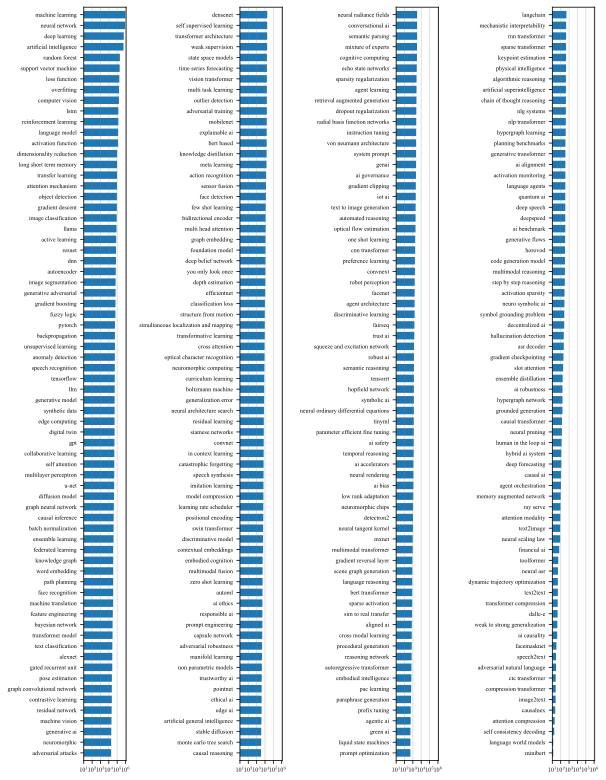
\includegraphics[height=0.95\textheight, keepaspectratio]{logarithmic_bar_graph_seach_term_document_count.pdf}
		\vspace{1em}
		\caption*{\small\textit{Sorted logarithmic bar graph of retrieval counts for the 279 query terms used to construct the AI corpus from OpenAlex. Each bar represents the number of works returned by an individual term; terms were curated to be AI-specific and to avoid redundancy via subsumption. The y-axis is on a log\textsubscript{10} scale to accommodate the heavy-tailed distribution, preserving comparability across orders of magnitude.}}
		\label{fig:keyword_log_bar_graph}
	\end{center}
}]



\subsection{Quality Control and Postprocessing}

After downloading and deduplication, the database contained \textbf{3{,}346{,}705} works. Not all records can contribute to our research questions, so we first assessed metadata completeness for key fields. 

\begin{figure}[H]
	\centering
	\caption{\textcolor{darkergray}{Metadata completeness of initially downloaded OpenAlex dataset}}
	\includegraphics[width=\columnwidth]{resources/completeness_bar_graph.pdf}
	\label{tab:metadata_completeness_initial_dataset}
\end{figure}


As shown in \figurename~\ref{tab:metadata_completeness_initial_dataset} in spite of performing better scores than expected based on the Table~\ref{tab:skg_comparison}, the country of origin field is the primary bottleneck with a completeness of 64.3\%. Inferring national attributions ex post (e.g., from names, language, funders, or publishers) would introduce unknown biases; therefore, records without a country attribution were removed. For downstream analyses, every retained record must provide (i) an abstract for topic modeling, (ii) a country of origin for geographic attribution, and (iii) at least one indicator for authority estimation—either cited\_by\_count or referenced\_works. Since cited\_by\_count is complete (100\%), records lacking references but meeting (i) and (ii) were kept. Likewise, missing doi or title did not trigger exclusion if the other criteria were satisfied.

From the authors' institutional affiliations, a \textit{country of origin} variable was derived. This variable captures the geographic distribution of all contributing author institutions per work, represented as a list of tuples containing country codes and their respective shares of total author institutions. For example:
\begin{center}
	\texttt{[("CN": 0.5), ("US": 0.25), ("DE": 0.25)]}
\end{center}
indicates that 50\% of the authors work in institutions located in China (not neccessarrily financed by China), 25\% in the United States, and 25\% in Germany. This representation facilitates nuanced analyses of international collaboration patterns and geographic contributions at the institutional level.

For abstracts, three additional quality rules were applied:
\begin{enumerate}
	\item \textbf{Language filter:} Only English abstracts were retained to avoid machine translation artifacts. Non-English (including unknown) constituted \textbf{4.64\%} (155{,}430 works) overall; among these, Spanish and Portuguese accounted for \textbf{2.61\%} (73{,}726 and 13{,}736), and Indonesian for \textbf{0.57\%} (19{,}008). Given the study’s global scope and the small relative share, excluding non-English text is acceptable and improves textual comparability.
	\item \textbf{Length normalization.} Extremely short or very long abstracts distort the embedding space. Therefor \textbf{107{,}515} records with abstract lengths below 100 and above 1000 token were removed. 
\end{enumerate}

%The follwing \figurename~\ref{abstract_distribution_histogram} shows the distribution of abstracts lengths after the removal of rows whose couldnt be assigend to any country.
%\begin{figure*}[!t]
%	\centering
%	\caption{Abstract token length distribution}
%	\vspace{1em}
%	\includegraphics[width=\linewidth]{resources/abstract_token_length_distribution_008.pdf}
%	\vspace{1em}
%	\caption*{\small\textit{This histogram shows the distribution of abstract lengths in tokens.
%			Very short abstracts below 100 token are either from conference papers and  or metadata artifacts
%			such as keyword lists or boilerplate entries.}}
%	\label{fig:abstract_distribution_histogram}
%\end{figure*}

After applying these filters, the final analysis corpus comprises \textbf{1{,}986{,}659} works of which 81.4 \% are articles, 11.1\% preprints, 3.7\% reviews, 1.6\% book-chapters, 1.7\% peer-reviews, 0.5\% dataset and 0.2\% dissertations. Including all document types in the analysis corpus is important because it avoids introducing selection bias by privileging specific formats such as journal articles over other recognized forms of scholarly communication.


\begin{figure}[H]
	\centering
	\caption{\textcolor{darkergray}{Metadata completeness of final OpenAlex dataset}} % optional
	\includegraphics[width=\columnwidth]{resources/working_dataset_completeness_bar_graph.pdf}
	\label{tab:metadata_completeness_wokring_dataset}
\end{figure}

As shown by \figurename~\ref{tab:metadata_completeness_wokring_dataset} the completeness of metadata is strongly correlated across fields, which means that the filtering of works lacking a country of origin also resulting in the improvement of the completeness of all other metadata. With 92.2\% the (outgoing) references are the new minimum. This dataset will be considered complete and not manipulated or aditionally filtered thorughout the diffrent layers of analysis. 


\twocolumn[{%
	\begin{center}
		\captionof{figure}{Dataset Construction Pipeline Diagram}
		\vspace{1em}
		\includegraphics[width=\linewidth]{data_extraction_pipeline_diagram.pdf}
		\label{dataset_construction_pipeline_diagram}
		\vspace{2em}
	\end{center}
}]




\section{Methodology}

The methodological framework of this study is divided into two complementary domains, directly aligned with the research questions. 

First, a semisupervised and hierarchical topic modeling approach is applied to the titles and abstracts of all works contained in the curated dataset. The objective of this stage is to combine the strengths of algorithmic separation and human understanding of semantic coherence to identify latent subdisciplines within the broader field of AI research.

Second, the study quantifies the relative research authority of individual countries within the subdisciplines identified in the first stage. This is accomplished through a citation-network analysis that computes centrality measures for the most recent research outputs. By constructing directed citation graphs and analyzing their topological properties, the study derives metrics of scholarly influence and connectivity, thereby providing an empirical basis for assessing the international distribution of research leadership in AI. In the following sections these two methodological components are described in detail.


\subsection{Subdiscipline Retrieval}


The identification of AI subdisciplines is conducted through a hierarchical, semi-supervised topic modeling pipeline. The overall procedure consists of three main steps: (i) vectorization of texts into a numerical representation, (ii) clustering and exploration of the thematic space, and (iii) expert-guided consolidation and propagation of cluster labels. This design combines algorithmic discovery with human interpretation, ensuring that the final hierarchy combines bottom up discovery of unexpected clusters while perserving semantically meaningful and cohesive clusters through top-down labeling.

\subsubsection{Vectorization}

In order to identify cohesive clusters of AI subdisciplines, the corpus must first be transformed into numerical representations that make the structure of the data accessible both to algorithms and to human interpretation. The purpose of these representations is not only to position works in a common semantic space where distances and proximities can be quantified, but also to provide interpretable cues that enable an expert to evaluate whether the resulting clusters correspond to meaningful subfields. To achieve this, two complementary forms of vectorization are applied in parallel. Dense transformer embeddings (SPECTER) provide a compact representation optimized for geometry, allowing documents to be visualized in UMAP space and grouped by clustering algorithms. Sparse TF–IDF features, in contrast, retain a transparent link to the underlying vocabulary and make it possible to extract distinctive keywords that characterize each cluster. Together, these representations give the expert both a “map” of the corpus (geometric structure) and a “lexicon” of its contents (vocabulary cues), ensuring that consolidation decisions are grounded in both statistical proximity and semantic interpretability. For each work, the text input is constructed by concatenating the title and abstract, and since both models are robust to raw scientific text, no additional preprocessing such as stop-word removal or lemmatization is applied. 

For geometric representation, the SPECTER model is employed. SPECTER is a transformer-based encoder trained on scientific citation networks to produce dense semantic embeddings of papers from their titles and abstracts. \cite{cohan2020specter} Each document is tokenized into overlapping windows (100 tokens, stride 50), with chunk-level embeddings averaged to obtain a single 768-dimensional vector per work. Since it is trained directly on the same type of text available in our dataset (titles and abstracts), SPECTER suits our requirements perfectly. These dense embeddings capture higher-level semantic similarity between documents and provide a compact basis for geometric operations such as UMAP projection and KMeans clustering.  

In parallel, a sparse vocabulary-based representation is created using \texttt{scikit-learn}’s \texttt{TfidfVectorizer}. \cite{pedregosa2011scikit} This method constructs a document–term matrix in which each dimension corresponds to a unique token or token $n$-gram retained by the pipeline. The resulting matrix \(X \in \mathbb{R}^{N \times D}\) has $N$ documents and a feature dimensionality equal to the size of the extracted vocabulary, typically on the order of $10^{6}$. While extremely sparse, such matrices remain computationally tractable and allow the ranking of terms by their relative importance across clusters. Unlike SPECTER, the TF–IDF representation is fully transparent and interpretable, making it particularly suited for deriving distinctive cluster labels.  

Together, these two representations complement each other: SPECTER embeddings provide the geometric structure necessary for clustering, while TF–IDF features supply the interpretable vocabulary that enables experts to understand and validate the resulting clusters.



\subsubsection{Clustering}

Once documents have been vectorized, the next step is to identify groups of them that represent coherent research fronts. This is achieved in two complementary ways: (i) clustering of dense SPECTER embeddings to detect structure in semantic space, and (ii) TF–IDF keyword analysis to provide interpretable labels for each cluster.

\paragraph{Clustering with SPECTER embeddings.}  
The dense SPECTER representations are used as the geometric basis for clustering. First, the high-dimensional embedding space is projected into two dimensions using UMAP (metric = cosine, $n\_neighbors = 15$, $min\_dist = 0.1$) to support visualization. Outliers are removed with an Isolation Forest (contamination = 0.01), and UMAP is recomputed for a clearer layout.  

Clustering is performed with KMeans. To evaluate the appropriate number of clusters, the silhouette score was computed across a wide grid of \(k\) values. The results showed no clear peak, suggesting that the data do not contain a single internally optimal partition. This aligns with broader concerns that data-driven heuristics for “optimal” \(k\) are often fragile and prone to post-hoc rationalization.\cite{bulatov2024determination} For this reason, \(k\) is treated as a tunable hyperparameter guided by interpretability rather than statistical heuristics. A relatively high value (\(k = 50\)) is selected to deliberately over-segment the corpus, preserving small but meaningful research fronts. These fine-grained clusters provide the raw material for subsequent expert consolidation into a smaller number of thematically coherent superclusters.


\paragraph{TF–IDF cluster labeling.}  
While SPECTER embeddings provide a robust geometric basis for clustering, they are inherently opaque to human readers: the dimensions of the embedding space do not correspond to interpretable terms. To render the 50 clusters generated in the embedding space intelligible, a complementary TF–IDF analysis is applied. For each cluster, the relative importance of terms is evaluated using a combined distinctiveness–representativeness criterion. Distinctiveness refers to the ability of a term to differentiate a given cluster from all others, while representativeness reflects how well the term characterizes the thematic scope of the cluster itself. By ranking vocabulary items under this heuristic, the ten highest-scoring keywords are selected to form a concise label for each cluster. These keyword labels do not constitute the final subdiscipline names, but rather provide interpretable cues that guide the expert assessment and subsequent consolidation of clusters into thematically coherent superclusters.



\subsubsection{Cluster Consolidation}

The fifty fine-grained clusters produced in the SPECTER embedding space serve only as a provisional partition. In the next stage, a human expert evaluates these clusters and consolidates them into a smaller number of semantically coherent superclusters. This step operationalizes the semi-supervised philosophy of the pipeline: algorithmic methods generate structure at high resolution, while human judgment ensures that the resulting categories align with meaningful subfields.

To support this process, the embedding space is projected into two dimensions with UMAP and rendered as an interactive visualization. The interactive chart allows clusters to be toggled on or off, inspected via hover-over tooltips displaying cluster labels, and explored through zoom and pan controls. This interface enables the expert to focus on specific regions of the landscape, compare cluster proximities, and assess potential overlaps or thematic boundaries.

Alongside the visualization, each cluster is annotated with its TF–IDF-derived keyword label. This combination of geometric layout and interpretable vocabulary provides the expert with multiple perspectives for making consolidation decisions. Clusters judged to reflect variations of the same research front are merged, while small but distinctive clusters are preserved as separate categories. The outcome is a thematically coherent set of superclusters that balances the fine resolution of algorithmic partitioning with the interpretability required for downstream scientometric analysis.

Once the expert-defined superclusters are finalized, a deterministic mapping is created that assigns each of the fifty initial cluster IDs to its corresponding supercluster. This mapping ensures that the consolidation process is fully transparent and reproducible. Using this mapping, all works in the dataset are relabeled: each document inherits the supercluster assignment of its original cluster. To facilitate downstream analysis, only numerical codes are used for the superclusters, and these codes are written directly into the project’s SQLite database. This guarantees a consistent, machine-readable representation of the human-curated subdiscipline structure across the full corpus.

\subsubsection{Hierarchical Structure}

The clustering and consolidation procedure described above is not performed only once but repeated in a hierarchical manner. After the initial run, which partitions the entire corpus into a small number of broad domains (H1), each resulting supercluster is taken as a new input space and subjected to the same sequence of steps: vectorization, high-$k$ clustering, TF–IDF labeling, interactive visualization, and expert consolidation. This second iteration produces a more fine-grained partition of each domain into meso-level subfields (H2).  

The process is then applied a third time within each H2 cluster, again combining algorithmic segmentation with expert review, yielding micro-level research fronts (H3). At each stage, the principle remains the same: begin with an over-segmented clustering to expose fine topical resolution, and then rely on human judgment supported by interpretable cues to consolidate them into thematically coherent units.  

This recursive application creates a consistent three-level hierarchy of subdisciplines. The H1 layer captures broad disciplinary domains, the H2 layer organizes them into meso-level thematic clusters, and the H3 layer identifies specific research fronts. The hierarchical design enables analysis at multiple resolutions, from high-level disciplinary comparisons down to the granularity of individual research niches, while maintaining interpretability and auditability across all levels.

\subsubsection{From Subsample to the Full Corpus}

Processing the entire corpus of nearly two million works with dense SPECTER embeddings was computationally prohibitive. To make the procedure feasible, the clustering pipeline was therefore applied to a random subsample of 100,000 documents. This reduction preserves the statistical diversity of the dataset while keeping resource requirements manageable, but it raises the challenge of how to extend the expert-defined superclusters obtained from the subsample to the complete corpus.  

To address this, a reference set was constructed for each of the $k=50$ initial clusters. Specifically, 20 \emph{central} abstracts (closest to the cluster centroid in embedding space) and 100 \emph{random} abstracts were extracted per cluster. These reference texts, together with their TF–IDF labels and assigned supercluster mappings, form a compact but representative anchor set.  

Once expert consolidation had been completed on the subsample, the reference embeddings were used to propagate labels to all two million works. Each document in the full corpus was embedded with SPECTER and assigned to the most similar item in the reference set by cosine similarity. Through this mechanism, every work in the dataset could be attributed to one of the predefined $k=50$ clusters and, via the deterministic mapping, to its corresponding supercluster. This approach ensures computational feasibility while maintaining consistency and reproducibility of the labeling across the full corpus.


\twocolumn[{%
	\begin{center}
		\captionof{figure}{Topic Modeling Pipeline Diagram}
		\vspace{1em}
		\includegraphics[width=\linewidth]{topic_modeling_pipeline_diagram.pdf}
		\label{topic_modeling_pipeline_diagram}
		\vspace{2em}
	\end{center}
}]




\subsection{National Research Authority}

A central aim of this study is to measure the distribution of research authority in artificial intelligence across the globe. Authority is understood here as the relative influence of research outputs within their scientific context, approximated through bibliometric indicators. Several quantitative metrics exist to capture such influence, but their suitability depends strongly on data availability and comparability. Citation-based measures are relatively robust and consistent across regions, while network-based centrality indicators are often distorted by structural differences such as the prevalence of cross-border collaborations, variation in the number of authors per paper, and unequal densities of research institutions. For this reason, the emphasis is placed on normalized citation-based metrics, complemented by additional indicators to provide a balanced perspective.

\textbf{Countries and political blocs:}  
The analysis does not focus exclusively on individual nation states. Geopolitical aggregates play an increasingly important role in global technological competition and policymaking, and their inclusion provides a more accurate picture of power dynamics. Eight major blocs are therefore considered alongside individual countries:  

Therefore, regional integration organizations are also included in the analysis, namely the European Union (27 members), the African Union (55), the Association of Southeast Asian Nations (10), the Southern Common Market (5), and the Gulf Cooperation Council (6). In addition to these regional frameworks, BRICS+ (10) is considered. Finally, the OECD (38) and the G-77 (134) are included as a proxy for the “Global North” and the “Global South.” These categories are not perfect, as 21 states (including several post-Soviet, island, and micro-states) are members of neither, and three countries (Chile, Colombia, Costa Rica) hold dual membership.


\subsubsection{Normalized Citations}

Citations remain the most widely recognized proxy for scholarly influence. To adjust for differences in publication year and subdiscipline, raw counts are normalized relative to the mean of comparable works. For a paper \(p\) in subdiscipline \(s\), published in year \(t\), the normalized citation score is defined as:

\begin{equation}
	\text{NormCitations}_{p,s} = 
	\frac{
		\text{Citations}_{p}
	}{
		\text{MeanCitations}_{t,s}
	}
\end{equation}

This adjustment corrects for the fact that older papers have had more time to accumulate citations and that citation densities differ across research areas. Normalized citation scores thus provide a fairer comparison across time and disciplines.


\subsubsection{Normalized Centrality}

Beyond raw citation counts, influence can also be approximated through a paper’s structural position in the citation network. Centrality measures such as PageRank capture not only direct citations but also indirect influence through chains of references. For a paper \(p\) in subdiscipline \(s\), the normalized centrality is given by:

\begin{equation}
	\text{NormCentrality}_{p,s} = 
	\frac{\text{Centrality}_{p}}
	{\text{Mean}(\text{Centrality}_{s})}
\end{equation}


While this approach provides additional nuance, its interpretability is limited. Cross-institutional collaborations, differences in author counts, and uneven institutional networks can heavily skew centrality measures across regions, reducing comparability. For this reason, centrality is treated as a complementary, but not primary, measure of authority.


\subsubsection{Field-Weighted Citation Impact (FWCI)}

As a further bibliometric indicator, the Field-Weighted Citation Impact (FWCI) compares observed citation performance with the expected citation rate for similar publications. For a paper \(p\), FWCI is defined as:

\begin{equation}
	\text{FWCI}_{p} =
	\frac{
		\text{Citations}_{p}
	}{
		\text{ExpectedCitations}_{\text{field},t}
	}
\end{equation}

where the denominator reflects the average citation rate of works of the same type, field, and year. A value of 1 indicates performance at the global average, values above 1 indicate above-average impact, and values below 1 indicate below-average impact. FWCI is widely used in scientometric assessments because it accounts for both field-specific citation practices and temporal effects, allowing for meaningful cross-disciplinary and cross-national comparisons.


In sum, national and bloc-level research authority is measured through a combination of normalized citation scores, network-based centrality, and FWCI. This multi-metric approach balances robustness, comparability, and contextual nuance, enabling a more reliable assessment of how influence in AI research is distributed globally.


\section{Findings}
\label{sec:findings}
This section is structured around the two guiding research questions. RQ1 is addressed by presenting the hierarchical clustering of the AI corpus: from broad macro-domains to fine-grained subdisciplines, visualized through UMAP projections that highlight both cluster cohesion and their relative positions in the research landscape. RQ2 shifts the focus to the geopolitical dimension: national research authority is first assessed on the full dataset and then within these subdiscipline. Together, these complementary perspectives expose both the thematic architecture of contemporary AI research and the distribution of influence across countries and regions.

\subsection{Hierarchical Topic Modeling}
\label{sec:results_topic_modeling}

The following subsection introduces the hierarchical organization that emerged from the topic modeling of the AI corpus and outlines how it structures the subsequent analysis. The goal is to provide an overview of the resulting clustering architecture before examining, in the following parts, the geometric and semantic topology of the field in greater depth.

As can be seen in \figurename~\ref{fig:exemplar_clustering_hierarchy}, the topic modeling assigns each work to one of three hierarchical levels. The model distinguishes 5 macro-clusters, 31 meso-clusters, and 106 micro-clusters. Each micro-cluster has a direct parent in a meso-cluster and a grandparent in a macro-cluster; conversely, every macro-cluster can be decomposed into its meso- and micro-components. This nested structure enables analysis across multiple scales of granularity, from the broad disciplinary domains that define the outer architecture of AI research down to the fine-grained research fronts where methodological and thematic convergence occurs.

The following subsections build upon this hierarchy to examine the internal topology of the AI research landscape. They analyze how clusters relate spatially in the embedding space, where overlaps or boundary zones appear between domains, and how the underlying term distributions shape the semantic contours of each area. In doing so, the analysis integrates both geometric and lexical dimensions to describe the multi-layered structure of contemporary artificial intelligence research.


\twocolumn[{%
	\begin{center}
		\captionof{figure}{Exempular Clustering Hierarchy}
		\vspace{1em}
		\includegraphics[width=\linewidth]{resources/h1_h2_h3_clustering_example.pdf}
		\vspace{1em}
		\caption*{\small\textit{Cluster granularity increases from left to right, with lighter hues denoting higher-level, semantically broader groupings. Each cluster is mapped to a corresponding level within the hierarchical taxonomy illustrated above, from domain-wide classifications (e.g., Computer Science) to fine-grained subdomains (e.g., Image Generation and Segmentation).}}
		\label{fig:exemplar_clustering_hierarchy}
		\vspace{2em}
	\end{center}
}]

% \twocolumn[{%
%	\begin{center}
%		\vspace{-3em}
%		\captionof{figure}{Mesocluster UMAP}
%		\vspace{1em}
%		\includegraphics[width=\linewidth]{resources/100k_mesocluster_visulization_greybox.pdf}
%		\vspace{1em}
%		\caption*{\small\textit{Explaination of why there is extensive 	overlapse, -> UMAP does that when projecting highdimensional data on 2D space and also clustering was done not only using UMAP clusterings but also the TFIDF Labels.}}
%		\label{fig:mesocluster_umap_with_legend}
%		\vspace{2em}
%	\end{center}
%}]



\subsubsection{Topology}

The Topology of the cluster visualization can be interpreted in the following ways: first there is the size of the clusters which is proportionate to the number of works inside that cluster and thus represents the relative attention this field of research has attracted from 2020 to 2025. secondly there is the relative position of the clusters, which reveals semantic proximity and differences. Especially the more granular clusters and their names can thus show research proximity even across the borders of macro clusters or show which micros are centered whithin which mesos and macros. Yet one has to be careful: as the abstracts and titles used for the embeddings contain words transporting both the domain vocabulary AND the methodology, which cannot be differentiated from the UMAP. 


\paragraph{H1 Hierarchy}
The five clusters of the H1 topic modeling consist of (0)~Computer Science, (1)~Biomedical Science, (2)~Social Science, (3)~Natural Science, and (4)~Engineering. As can be seen from the relative position of the clusters, the Computer Science cluster is most central, as it represents the methodological core of AI research—the locus where novel architectures, algorithms, and learning paradigms originate. The other four macro-clusters can be interpreted as domain-specific translations of this core, where computational techniques are adapted to distinct epistemic environments. Their arrangement in the embedding space reflects this gradient: Engineering and Natural Science remain topologically adjacent to Computer Science, forming a contiguous basin of applied methodological research, whereas Biomedical Science and Social Science occupy more peripheral positions that correspond to the integration of AI into empirical and reflexive knowledge regimes. The partial overlaps between Computer Science, Engineering, and Natural Science thus indicate zones of methodological exchange—areas where innovations in model design, optimization, or data representation circulate most rapidly across disciplinary boundaries. In contrast, the relative distance of Social Science marks AI’s expansion into interpretive and normative terrains, where computational methods increasingly intersect with governance, ethics, and policy analysis.


\paragraph{H2 Hierarchy}
The 31 clusters of the H2 hierarchy further subdivide the 5 macro-clusters into thematically coherent meso-domains, ranging from five to seven per macro-domain. At this level, the structure becomes markedly more heterogeneous and reveals the internal organization of each disciplinary basin. Some meso-clusters correspond closely to established subfields—such as \emph{Natural Language Processing}, \emph{Medical Imaging}, or \emph{Autonomous Systems}—while others emerge as hybrid zones whose attribution to a single macro-domain is more interpretative than categorical. 

A prominent example is the \emph{Construction and City Planning} meso-cluster, which merges two neighboring micro-clusters centered on \emph{construction technology} and \emph{urban mobility}. Its geometry and vocabulary span both Engineering and Social Science: while construction research draws on material science, statics, and durability modeling, urban planning invokes demographic and behavioral data, governance models, and environmental simulation. The resulting overlap produces a semantically dense interface where technical optimization and social coordination intersect. Similar ambiguities occur in the \emph{AI Governance and Ethics} meso-cluster, which lies between Computer Science and Social Science and combines methodological debates on explainability with normative questions of accountability and bias. Another example is \emph{Energy Systems Optimization}, a meso-cluster connecting Engineering and Natural Science through shared concerns with control theory, grid forecasting, and sustainability modeling. On the other hand the Health Science Mesoclusters are rather peripheral with only Neuroscience showing significant overlapse with computer science Macro.

Such hybrid formations underscore the interpretive nature of the hierarchy: the meso-level does not merely partition the corpus but exposes points of epistemic convergence where AI methods migrate across disciplinary regimes. In this sense, the H2 hierarchy functions as a cartography of translation zones—regions that reveal how artificial intelligence operates not only within but also between its host sciences.


\paragraph{H3 Hierarchy}
The 106 micro-clusters constitute the most granular layer of the hierarchy and delineate active research fronts within the broader thematic basins of the H2 level. Each micro-cluster aggregates publications that share not only vocabulary and methodological framing but also, in many cases, data modalities, benchmark tasks, or technical pipelines. This level thus captures the operative scale of AI innovation—the sites where new architectures, datasets, and applications emerge before diffusing upward into meso- and macro-domains.

While many micro-clusters remain firmly embedded within their respective disciplinary domains, others act as connective tissue between them. For instance, the \emph{Molecular Biology and Drug Discovery} micro-cluster, nested within the Biomedical domain, draws upon both biological ontology and computational chemistry, forming a boundary region with the Natural Sciences. Similarly, \emph{Neuromorphic Hardware Accelerators}, positioned under Engineering, reflects the convergence of materials science, electrical engineering, and computer architecture, translating algorithmic principles into physical substrates. On the methodological side, \emph{Cybersecurity and Adversarial Robustness} occupies a central position within the Computer Science basin, where theoretical models, security protocols, and machine-learning optimization coalesce around shared technical challenges. Other clusters—such as \emph{Remote Sensing and Environmental Modeling}—extend across macro-domains by linking Natural Science data infrastructures with AI-driven geospatial analysis, again demonstrating how micro-level specialization facilitates interdisciplinary transfer.

These examples illustrate how the H3 layer transforms the abstract structure of the hierarchy into a dynamic landscape of knowledge production. Here, proximity in embedding space often reflects the circulation of methods, datasets, or evaluation paradigms rather than simple topical similarity. The micro-clusters therefore reveal the fine-grained topology of the field: dense cores of algorithmic development surrounded by a periphery of domain-specific applications, together forming the dynamic interface through which AI research continuously redefines its disciplinary boundaries.



\subsubsection{Naming}

Many of the names attributed to the clusters do not neccesarrily show any connection to AI or even computer science and practically all of them have already and still do exist without AI adoption. Yet the names are mainly chosen to allow for differrentioation of clusters with a sufficient level of topological and geografic distinction. When measured against the categories attibuted to the works by OpenAlex we can see though that social science only makes up 10.4 \% yet it covers 18.8\% in the H1 clustering. That excess is largely at the expense of the computer science category which is attributed to 30.8\% by OpenAlex and only 22.2\% in this paper. A look in OpenAlexes more granular fields reveals that the difference comes mainly form the attribution of Communication \& Media Studies, AI Ethics and Decision Science to social science in our case and to computer science in the case of OpenAlex. 


\twocolumn[{%
	\begin{center}
		\vspace{-3em}
		\captionof{figure}{Cluster Summarization UMAP}
		\vspace{1em}
		\includegraphics[width=\linewidth]{summarized_cluster_umap_2025_09_11.pdf}
		\label{cluster_summarization_umap}
	\end{center}
}]



\subsection{National AI Research Authority across complete Dataset}

Before analyzing authority within specific subdisciplines, it is essential to establish a baseline assessment of global research dominance across the complete AI corpus. Examining the total dataset provides a foundational reference against which all subsequent, more granular comparisons can be contextualized. It captures the aggregate distribution of research capacity, collaboration, and citation impact across countries and blocs, offering a macroscopic view of where scholarly influence is concentrated. This global overview serves as the analytical groundwork upon which the subdisciplinary decomposition in later sections is built, ensuring that variations observed within individual fields can be interpreted relative to the overall structure of AI research.



\subsubsection{Geomapping of Total Citation Distribution}

To provide an initial overview of the global research landscape, \figurename~\ref{logarithmic_distribution_citation_sum} presents a world map of aggregated citation counts. The figure reveals a strong geographical concentration of research influence. Publications originating from China account for the highest number of citations, totaling 4,728,364, followed by the United States with 3,648,720. The next ranks are occupied by the United Kingdom (1,220,273), Germany (876,943), and India (787,853). When aggregated, the European Union (EU-27) reaches 4,079,623 citations. The Association of Southeast Asian Nations (ASEAN) would occupy the sixth position—behind India but ahead of Italy and Canada—with 711,580 citations. In contrast, Mercosur contributes comparatively little with 170,813 citations, and the African Union performs similarly modestly with 402,405 citations.
It is important to note that these regional results are partially affected by linguistic filtering (e.g., the exclusion of Spanish-language works), which likely underestimates the citation volume of Latin American countries.

On the global level, the inequality in the distribution of AI-related research output is substantial. The population-weighted Gini coefficient for total AI citations amounts to 0.665, exceeding that of nominal GDP (0.632) and, even more distinctly, purchasing-power-parity–adjusted GDP (0.450). This comparison demonstrates that the global geography of AI knowledge production is an exceptionally unequal and hierarchical system, in which scientific influence is concentrated in a small number of countries to an even greater extent than economic wealth.

When comparing the relative national shares of AI citations to each country’s share of global GDP (PPP-adjusted), a distinct geography of over- and underperformance emerges. The most pronounced outliers are found in Europe, where several smaller or innovation-driven economies exceed their expected citation volume by large margins: Finland produces 3.70 times its global economic share, followed by Switzerland (3.47), the United Kingdom (2.86), Denmark (2.61), Sweden (2.48), and the Netherlands (2.42). Beyond Europe, strong overperformers include Australia (2.72), Canada (2.03), Israel (2.44), and Singapore (2.37). The two global research powerhouses, the United States (1.26) and China (1.15), perform roughly in proportion to their global economic weight.
On the lower end of the distribution, countries such as India (0.51), Japan (0.46), and Indonesia (0.41) contribute only about half as much to global AI research as their PPP-based economic share would suggest. Larger economies like Mexico (0.18), Russia (0.16), and Argentina (0.12) are the weakest performers among the major economies.

When using nominal GDP instead of PPP-adjusted GDP as the baseline, the picture shifts notably. Here, several OECD countries lose relative ground by a factor between 1.5 and 2, while emerging markets become more prominent. Iran leads the ranking, producing 2.7 times more AI citations than its nominal GDP share, followed by Pakistan (2.15) and Malaysia (2.15). Also noteworthy are Tunisia (1.91) and Egypt (1.76), whose relative citation output reveals growing ambitions in the field. In this perspective, China (1.33) slightly surpasses and the United States (0.69) falls below their economic shares, while India (1.19) and Indonesia (0.78) perform roughly in line with their nominal GDP. Japan (0.41), Russia (0.32), and Mexico (0.20) remain the lowest-performing major economies in both frameworks.

Both PPP-adjusted and nominal GDP comparisons are essential, as they capture different dimensions of global economic power.
Nominal GDP, expressed in current international dollars, reflects a country’s financial capacity in global markets and its ability to fund research competitively through internationally valued currencies. PPP-adjusted GDP, by contrast, accounts for domestic purchasing power, offering a better proxy for real economic activity and the potential scale of internal R\&D ecosystems.
Comparing AI research output against both measures therefore distinguishes between internal capacity for innovation (PPP perspective) and external competitiveness in the global knowledge economy (nominal perspective). The divergence between the two highlights how some emerging economies achieve research overperformance relative to their domestic resources, whereas advanced economies often leverage stronger global purchasing power but show lower proportional efficiency in AI-related knowledge production.



\twocolumn[{%
	\begin{center}
		\captionof{figure}{Logarithmic distribution of AI publications by country}
		\vspace{1em}
		\includegraphics[width=\linewidth]{country_contributions_aitoff_log.pdf}
		\caption*{\small\textit{Aitoff projection of the world map displaying the logarithmic distribution of national citation totals. For each work, citations are fractionally attributed to all contributing countries according to author–affiliation shares, and then aggregated at the country level. Citation counts are shown on a log\textsubscript{10} scale to account for the strong skew between high- and low-impact nations.}}
		\label{logarithmic_distribution_citation_sum}
	\end{center}
}]

\subsubsection{Multidimensional Performance Heatmap}

\figurename~\ref{fig:research_performance_heatmap} displays the research performance of the twenty most publishing countries alongside aggregated indicators for eight major international blocs. The first five columns (publication share, citation share, top-10\%, top-1\%, top-0.1\%) report each country’s fractional contribution to the global AI research corpus, while the subsequent rate-based indicators—average citations, zero-cited rate, collaboration rate, and open-access rate—describe the internal distributional characteristics within each national publication portfolio.

To preserve interpretability across different scales of performance, the figure is divided into two sections: one for countries and one for international blocs. The Viridis color scale is normalized separately for each section, ensuring that the high citation densities of the Global North and the lower aggregate volumes of the Global South do not compress all values into the lower end of a single shared color range. This independent normalization allows for a meaningful differentiation of relative strengths and weaknesses within each group, rather than visually biasing the comparison toward the dominant producers.

\twocolumn[{%
	\begin{center}
		\vspace{-3em}
		\refstepcounter{figure}
		\captionof{figure}{12-dimensional research-performance matrix of 20 most publishing countries and 8 organizations}
		\vspace{0.5em}
		\includegraphics[width=\linewidth]{heatmap_top_20.pdf}
		\vspace{1em}
		\caption*{\small\textit{Citation inequality is measured via the Gini coefficient of each country’s citation distribution. Growth rate corresponds to the compound annual growth rate (CAGR) of fractional publication counts between 2020 and 2023, with 2024 excluded due to incomplete data coverage. Field impact is calculated as the ratio of observed citations to expected citations after normalizing by publication year and H3-level field averages, thereby identifying over- or under-performance relative to global baselines.}}
		\label{fig:research_performance_heatmap}
	\end{center}
}]



\paragraph{publication share:} The Matrix confirms the head-heavyness of the distribution of publications. Four countries cover more than half of publications (51.5\%). 25.2\% of all AI publications are published by authors from Chinese institutions. Behind it is the US with 15.2\%. No other nation performs double digit percentages, but taken as a bloc the EU-27 contributes 18.5\%. Interestingly, Global North (OECD) and Global South (G77) are very close with 50.2 and 47.3 \% respectively.

\paragraph{citation share:} The citation aggregates are even more concentrated with 53.4\%. India slips to fifth rank, overtaken by the United Kingdom and Germany. The share of OECD countries thereby grows to 58.8 \% while the G-77 shrinks to 39.9 \%. 

\paragraph{top \% shares:} The three columns of the highest percentile papers show an intensification of research perfromance concentration. India, Indonesia and all other non-European countries except the US show consistent decline from their publication share to the top 0.1 percentile. In case of Indonesia the factor of underproportionality is 2000\%, 930\% for Russia, 353\% for Brazil and 218\% for India. Meanwhile the four big anglophone contributers, the US, the UK, Canada and Australia as well as Germany and Switzerland are the biggest profiteurs when compared to their publication share with Australia expanding their share of top permille papers by 197\% compared to their total publication share. While the US is still behind China in top-10\% and top-1\% papers it overtakes China with 538 (27.1 \%) of the 1987 most cited papers. OECD countries cover 65.1\% of top-0.1\% papers and the G-77 34.2\%. 

\paragraph{average citations:} The average citations is the first column that does not show national percentages of the full dataset and therefore its distribution is far from the ranking that is based on the publication share. The differences of national averages are considerable with Indonesia showing the minimum of the 20 countries with 3.5 citations per work while australia leads with 15.2. EU-27 countries fluctate across the average of 11.42, while the US has 12.4 and China 9.7, which is significantly lower than the OECD average of 11.9 yet significantly higer than the G-77 average of 8.56 which is especially pulled down by Indias average of 6.1 citations per work. Beyond that the performance of the GCC (Gulf Cooperation Council) which consists of Saudi Arabia, UAE, Oman, Kuwait, Qatar and Bahrain is remarkable with an average of 13.3. Yet with 1.5 \% of the total publications no single GCC country is represented in the top 20 list.

\paragraph{zero-cited rate:} After we located the most successfull papers we now turn to the least successfull: those which were never cited. One has to watch out, because the numbers are a snapshot of the downloading date in June 2025 and that means that the most recent papers of the dataset were only 6 months published and therefore had very little time to accumulate citations. Low values can therefore partly be explained by high growth rates which indicate overproportionality of newer papers over older ones. Yet results are largely consisten with the average citations contributing to the assumption of national citation - (skewed) continuous distribution. Russia (37.6), India (36.0) and Indonesia (38.7) again stand out with large percentages whereas EU-27 countries (23.1), South Korea (22.9) and Australia (20.5) show the lowest numbers. China (27.7) and the US (27.1) both score mediocre in this performance metric and therefore the difference between OECD (25.2) and G-77 (29.9) is smaller than in most previous comparison.

\paragraph{citation inequality:} The Gini-Coefficient shows that academia is a winner takes all game across the world. As desribed in the metthew effect often cited papers are often more visible and more trusted and therefore chosen more often as reference afterwards. Therefore all countries have very high citation inequalitys of more than 0.7. There is little regional or organizational consistency with the EU-27 scoring best with 0.74 and ASEAN worst with 0.80. China and the US score similarily high with 0.77 and 0.79 respectively. Canada shows the most unequal citation distribution among the 20 most publishing countries with 0.80.

\paragraph{growth rate:} The compound annual growth rate was calculated on the first 4 years of the corpus because there is some delay between publication and integerations in SKGs like OpenAlex which renders the 2024 data incomplete and thus prone to distrort growth rates. The growth rates of Ai-related publication are positive for all 28 entities. The five countries with the highest rates are all Asian with India and Indonesia taking the top spots. China is third with 23.3 \% while the US has the lowest rate with 4.4 \%. What this metric is not able to tell: 1. what percentage of overall research output of each country is related to AI. That means that it might be that the US already saturated AI research in 2020 while Asian countries are catching up with big strides. 2. What the overall reserach output growth. Maybe AI papers are just a latent variable of a greater tendency of Asian countries to develop their overall reserach output. The answer has to be a compromise between those two - clear is however that G-77 output grew with 23.2 \% while OECD countries grew with only 9.8 \%. 

\[
\text{CAGR} = \left(\frac{\text{publicationcount}_{2023}}{\text{publicationcount}_{2020}}\right)^{\tfrac{1}{4}} - 1
\]


\paragraph{international cooperation rate:} A work is considered \textit{international} when not all institutions of the publishing authors are located in the same country. International Collaborations is not only considered a marker of reserach quality and credibility but has proven to increase research quality by pooling resources, diversifying methodologies and exploiting network effects.  Yet one has to put into consideration that geographic and cultural proximity are not always best described by nation borders. A Cooperation between the Indian Institute fo Technology Madras in Chennai, Tamil Nadu and the University of Chandigarh, Punjab might satisfy the conditions of the theory better than a cooperation between TU Munich and TU Vienna even though only the latter is labeled as international cooperation.

The rates differ significantly across the globe. The European representatives fluctuate around 40\% while the US has 23.8, China 14.8, India 13.0 and Indonesia only 7.7. With 45.2 Switzerland has the highest score and is only overtaken by the GCC block which has a rate of 47.4 \% of international collaborations. Overall OECD countries have a clear edge over G-77 countries with 30.8 to 19.0 \%.

\paragraph{field impact:} A central metric in comparative scientometric analysis is the field-weighted citation impact (FWCI), which corrects for disciplinary differences in publication and citation practices. Raw citation counts are not directly comparable across fields, since, for example, biomedical sciences typically accumulate more citations than engineering or the social sciences. The FWCI normalizes each publication's citations by the expected citation rate of works in the same field, year, and document type. Formally, for a set of $N$ publications $p_i$ with citation count $c_i$ and expected citation baseline $e_i$, the metric is defined as
\[
\text{FWCI} = \frac{1}{N}\sum_{i=1}^{N}\frac{c_i}{e_i}.
\]
A value of $\text{FWCI}=1.0$ indicates that an entity's publications are cited at the world average for their fields, while $\text{FWCI}>1.0$ reflects above-average citation impact. In our results, the FWCI highlights the relative citation strength of countries and blocs independently of their disciplinary profile: large systems such as the United States and the European Union achieve values clearly above 1.0, suggesting sustained influence across diverse fields, whereas emerging contributors show lower FWCI values, reflecting either disciplinary skews towards less citation-intensive areas or genuinely lower international visibility.

\paragraph{open aceess rate:} The last metric of our research performace assessment captures the proportion of publications sthat are freely available to the global research community. This indicator is usually included in scientometrics because open access accelarates knowledge disseminations within academia and maximizes societal implementation. 

The open aceess rate range from Indias 49.8\% to the Netherlands 90.0\%. The EU-27s research is 84.9\% open access while the US stands at 74.5 and China at 62.9. Similarily OECD stands at 79.9\% and the G-77 at 66.0\%, yet that is mainly from the low scores of China and India. Other G-77 representatives like Indonesia (86.5\%), Brazil (77.7\%), Malaysia (81.4\%), Iran (70.0\%) and Russia (76.0\%) all feature values comparable to the EU-27 bloc.

\paragraph{conclusion:} The first five columns show national reserach performance in their absolute terms. Here China and the US are leading the globe by a large margin taking more than 40\% of the total in all metrics. Once taken together as EU-27 a third contender emerges and even overtakes the US in publication share, citation share and top-10\% share. Yet in top-1\% share and top-0.1\% they fall to third rank. In the other columns where we look on characteristics on a per publication basis rather than accumulating totals we see a diffrent pattern. OECD countries score consistenly better in average citations, feature less zero-cited publications, show more international collaboration, a higher field weighted citation impact and hgiher open acess rates compared to G-77 corpus. Yet the G-77 corpus is heavily impacted by the large shares of China and India and beyond that there are many excemptions. For example The six Gulf Monarchies of the GCC score highest among all 8 blocs in all but one (open-access) of the relative categories. 

\subsubsection{National Citation Percentile Distribution} 
While the preceding indicators each isolate specific aspects of performance — total publication volume, aggregate citation share, representation among the global top-percentile papers, average citations, and the zero-cited tail — they all implicitly reflect the underlying shape of how each country’s works are distributed across the global citation spectrum. The percentile distribution offers a compact way to visualize this continuum in a single profile, showing how national outputs are spread from the lowest quartile to the elite top-0.1\%. By normalizing citation counts within publication years, temporal bias is reduced, allowing for cross-national comparability of impact distributions rather than only headline shares. \figurename~\ref{fig:citation_percentile_distribution} synthesizes these dynamics for the twenty most prolific countries: nations with a broad upper-tail share of papers in the highest percentile bands stand out for disproportionate high-impact contributions, whereas left-heavy profiles reveal concentration in low-impact segments. In this sense, the distribution plot complements the earlier discrete metrics by providing a holistic view of national research impact across the full citation hierarchy.

\twocolumn[{%
	\begin{center}
		\vspace{-3em}
		\refstepcounter{figure}
		\captionof{figure}{National year-normalized citation percentile distribution (stacked bars)}
		\label{fig:citation_percentile_distribution}
		\vspace{1em}
		\includegraphics[width=\linewidth]{percentile_composition_top20_countries_plus_blocs.pdf}
		\vspace{1em}
		\caption*{\small\textit{Citation percentile distribution of the twenty most publishing countries (fractionalized by author affiliation) and eight international entities. Each horizontal bar represents an entity’s publication output normalized to 100\%, partitioned into six year-adjusted citation bands (0–25\%, 25–50\%, 50–75\%, 75–90\%, 90–99\%, 99–100\%). The year normalization ensures that publications of different ages are comparable despite varying citation accumulation windows. The inflated size of the lowest quartile reflects the fact that the global share of zero-cited papers frequently exceeds 25\%, thereby compressing the intermediate bands.}}
	\end{center}
}]


In order to complement absolute citation counts and bloc-level comparisons, we constructed a normalized citation percentile distribution for all countries and international entities. Each publication was assigned to one of six year-adjusted citation bands (0--25\%, 25--50\%, 50--75\%, 75--90\%, 90--99\%, 99--100\%), which allows publications of different ages to be compared despite varying citation accumulation windows. This year-normalization is particularly important because our dataset includes papers published up to just six months before scraping. Such recent outputs cannot yet display their long-term impact and, while some may later emerge as field-defining contributions, they presently register in the middle percentiles. This temporal effect compresses the extremes of the distribution: the lowest quartile is inflated by the global share of uncited works, and the uppermost percentiles underrepresent the ``winner-takes-all'' dynamic associated with the Matthew Effect. In consequence, the distributions should be read as an intermediate snapshot that is structurally biased toward the average, with exceptional outliers not yet fully visible.

Despite these caveats, the comparative results reveal important structural differences (Figure~\ref{citation_percentile_distribution}). China and the United States, the two dominant producers of AI-related research, are strikingly similar across the lower and middle percentile bands. Only at the very top does the United States maintain a modest advantage: its shares in the 90--99\% and 99--100\% citation strata are consistently larger, reflecting a slightly stronger concentration of globally leading publications. Europe (EU--27), by contrast, performs broadly on par with these two powers across the entire spectrum, confirming the bloc’s resilience despite being more fragmented institutionally. Smaller but research-intensive countries such as Australia, the United Kingdom, and Switzerland outperform in relative terms: they produce a disproportionately high share of papers in the top quartile and especially in the top decile, underscoring how well-resourced and internationally connected middle-sized systems can leverage quality over sheer output volume. In stark contrast, emerging systems such as India and Indonesia lag behind. Fewer than ten percent of their publications reach the global top quartile, pointing to an imbalance between rapid growth in publication volume and the slower development of internationally competitive impact.

The bloc-level comparison adds further nuance. The OECD as a collective still outperforms the G–77 in terms of high-percentile shares, but the gap is narrower than might be expected given historical patterns, indicating the increasing presence of high-quality research in the Global South. ASEAN and Mercosur exhibit heavily bottom-skewed distributions, with the majority of outputs located in the lower half of the citation spectrum, while BRICS+ performs more heterogeneously, largely driven by China’s outsized contribution. These findings suggest that while advanced economies retain a lead in producing highly cited research, the distribution of scientific excellence is slowly broadening. At the same time, structural and cultural factors mediate these outcomes: in Europe, the dense network of medium-sized universities encourages cross-border collaboration that disperses excellence more evenly, whereas in China and the United States, a small number of very large universities dominate, concentrating their citation power. Taken together, the percentile distributions confirm the dual dynamic already visible in the institutional network analysis: excellence remains concentrated in a few elite systems, but the gradual convergence of wider blocs signals a redistribution of impact across the global research landscape.


\subsubsection{Top 1000 Institutions}

In contrast to the preceding analyses that treated scientific production at the level of nation states, the present section disaggregates countries into their most influential \textit{institutions}. Specifically, we constructed a co-authorship network of the top--1000 institutions worldwide ranked by fractional citations. Each institution is assigned to one of four political blocs: \textbf{China}, the \textbf{United States}, the \textbf{EU--27}, and the \textbf{Rest of the World (ROW)}. The resulting network is laid out using the ForceAtlas2 algorithm, with node size proportional to an institution's cumulative fractional citations and edge weight reflecting the intensity of co-authorship (normalized by the number of participating institutions per work). To reduce visual clutter, only edges with a weight greater than or equal to 1.0 are displayed, while all edges were included in the layout simulation. We deliberately refrained from applying standard centrality metrics such as eigenvector, betweenness, or closeness centrality, since their interpretive validity is limited in the present context. These measures are highly sensitive to academic conventions and structural biases: for instance, smaller European universities tend to rely more strongly on cross-institutional and cross-border collaborations, which would artificially inflate their apparent centrality despite their comparatively modest citation weight. Similarly, U.S. or Chinese “megaversities” with strong internal capacities may appear less central simply because they collaborate less frequently across institutional boundaries, although they dominate in absolute research impact. Moreover, centrality scores are influenced by the density and granularity of national university systems (fragmented in Europe, consolidated in China), by language patterns that shape collaboration networks, and by disciplinary clustering that reflects field-specific norms rather than global influence. To avoid conflating these structural and cultural effects with genuine measures of research authority, we rely instead on the more transparent representation of institutional size (citations) and their direct co-authorship ties in the ForceAtlas2 layout.

\twocolumn[{%
	\begin{center}
		\vspace{-3em}
		\captionof{figure}{Global top-1000 institutions by citation-weighted collaboration network}
		\vspace{1em}
		\includegraphics[width=0.9\linewidth]{institution_network_top_1000_with_legend.pdf}
		\label{fig:cn_eu_us_top_1000_institutions}
		\vspace{2em}
		
		\tiny
		\setlength{\tabcolsep}{6pt}
		\renewcommand{\arraystretch}{1.12}
		\begin{tabular}{@{}l l l l l l@{}}
			\rc{1}{US}  & Stanford University &
			\rc{35}{CN} & Tongji University &
			\rc{69}{FR} & Centre National de la Recherche Scientifique \\
			\rc{2}{GB}  & University of Oxford &
			\rc{36}{SA} & King Abdulaziz University &
			\rc{70}{IT} & Sapienza University of Rome \\
			\rc{3}{CN}  & Chinese Academy of Sciences &
			\rc{37}{CH} & University of Zurich &
			\rc{71}{IT} & University of Padua \\
			\rc{4}{CH}  & ETH Zurich &
			\rc{38}{US} & University of Pennsylvania &
			\rc{72}{US} & Pennsylvania State University \\
			\rc{5}{GB}  & DeepMind &
			\rc{39}{CN} & University of Chinese Academy of Sciences &
			\rc{73}{US} & University of Illinois Urbana–Champaign \\
			\rc{6}{CN}  & Tsinghua University &
			\rc{40}{AU} & UNSW Sydney &
			\rc{74}{IT} & University of Bologna \\
			\rc{7}{AU}  & Monash University &
			\rc{41}{GB} & King's College London &
			\rc{75}{DE} & Ludwig\mbox{-}Maximilians\mbox{-}Universität München \\
			\rc{8}{GB}  & University College London &
			\rc{42}{NL} & Utrecht University &
			\rc{76}{US} & University of Wisconsin–Madison \\
			\rc{9}{US}  & Harvard University &
			\rc{43}{US} & University of California, San Diego &
			\rc{77}{DK} & University of Copenhagen \\
			\rc{10}{GB} & University of Cambridge &
			\rc{44}{US} & University of California, Los Angeles &
			\rc{78}{KR} & Seoul National University \\
			\rc{11}{US} & Massachusetts Institute of Technology &
			\rc{45}{NL} & Wageningen University \& Research &
			\rc{79}{US} & University of Florida \\
			\rc{12}{NL} & Delft University of Technology &
			\rc{46}{HK} & Hong Kong Polytechnic University &
			\rc{80}{GB} & University of Manchester \\
			\rc{13}{GB} & Imperial College London &
			\rc{47}{AU} & The University of Melbourne &
			\rc{81}{CN} & Chongqing University \\
			\rc{14}{CN} & Zhejiang University &
			\rc{48}{IT} & Politecnico di Milano &
			\rc{82}{NO} & University of Oslo \\
			\rc{15}{US} & University of Washington &
			\rc{49}{DK} & Technical University of Denmark &
			\rc{83}{IN} & Vellore Institute of Technology \\
			\rc{16}{CN} & Central South University &
			\rc{50}{CN} & Sichuan University &
			\rc{84}{US} & Georgia Institute of Technology \\
			\rc{17}{SG} & National University of Singapore &
			\rc{51}{NL} & University of Twente &
			\rc{85}{US} & Broad Institute \\
			\rc{18}{CN} & Wuhan University &
			\rc{52}{GB} & University of Edinburgh &
			\rc{86}{US} & University of California, Davis \\
			\rc{19}{US} & University of Michigan &
			\rc{53}{US} & Johns Hopkins University &
			\rc{87}{CN} & Xi'an Jiaotong University \\
			\rc{20}{CN} & Shanghai Jiao Tong University &
			\rc{54}{NL} & University of Groningen &
			\rc{88}{GB} & University of Glasgow \\
			\rc{21}{US} & University of California, Berkeley &
			\rc{55}{NL} & University of Amsterdam &
			\rc{89}{DK} & Aarhus University \\
			\rc{22}{NO} & Norwegian University of Science and Technology &
			\rc{56}{CN} & Harbin Institute of Technology &
			\rc{90}{US} & Columbia University \\
			\rc{23}{CN} & Peking University &
			\rc{57}{US} & Yale University &
			\rc{91}{CN} & Beijing Institute of Technology \\
			\rc{24}{HK} & University of Hong Kong &
			\rc{58}{GB} & University of Bristol &
			\rc{92}{US} & Carnegie Mellon University \\
			\rc{25}{DE} & Technical University of Munich &
			\rc{59}{US} & New York University &
			\rc{93}{US} & University of Southern California \\
			\rc{26}{CN} & Huazhong University of Science and Technology &
			\rc{60}{CA} & University of British Columbia &
			\rc{94}{US} & Cornell University \\
			\rc{27}{CN} & University of Electronic Science and Technology of China &
			\rc{61}{CN} & Fudan University &
			\rc{95}{NL} & Radboud University Nijmegen \\
			\rc{28}{CN} & Sun Yat-sen University &
			\rc{62}{CN} & Beihang University &
			\rc{96}{AU} & Queensland University of Technology \\
			\rc{29}{QA} & Qatar University &
			\rc{63}{CN} & Southeast University &
			\rc{97}{KR} & Sejong University \\
			\rc{30}{CA} & University of Toronto &
			\rc{64}{SA} & King Saud University &
			\rc{98}{BE} & Ghent University \\
			\rc{31}{CH} & École Polytechnique Fédérale de Lausanne &
			\rc{65}{JP} & The University of Tokyo &
			\rc{99}{AU} & The University of Sydney \\
			\rc{32}{US} & University of California, San Francisco &
			\rc{66}{AU} & The University of Queensland &
			\rc{100}{FI} & University of Helsinki \\
			\rc{33}{SG} & Nanyang Technological University &
			\rc{67}{CN} & Northwestern Polytechnical University & & \\
			\rc{34}{BE} & KU Leuven &
			\rc{68}{CA} & University of Waterloo & & \\
		\end{tabular}
	\end{center}
}]



The bloc distribution of institutions reveals distinct structural patterns: the EU--27 contributes \textbf{282 nodes}, China \textbf{213}, the United States \textbf{161}, and the Rest of the World \textbf{343}. In terms of total fractional citations, however, the distribution differs markedly. China accumulates the highest sum with \textbf{4.76 million citations}, followed by the EU--27 with \textbf{4.11 million}, the United States with \textbf{3.67 million}, and the Rest of the World with a comparatively dispersed but overall dominant \textbf{7.28 million}. This indicates that China's citation power is concentrated within a relatively smaller set of elite institutions, whereas Europe’s influence is spread more evenly across a larger number of universities and research centers. The United States likewise shows strong concentration, with comparatively few institutions capturing a disproportionately large share of citations. A structural factor behind these differences lies in the size of universities: both in China and the United States, the average number of students and professors per institution is substantially higher than in Europe, where higher education is more fragmented into smaller universities and specialized schools. In China this concentration has been actively promoted through the \emph{Project 211} and \emph{Project 985} reforms as well as the \emph{C9 League}, which together channeled resources into a small circle of comprehensive universities. In the United States, a similar elite stratum is represented by the Ivy League and the leading public research universities, which enroll tens of thousands of students each and employ several thousand faculty. Europe, by contrast, lacks a directly comparable pan-European grouping, although national excellence initiatives (e.g., Germany’s Excellence Strategy, France’s IdEx, or the clustering of Grandes Écoles) have sought to consolidate and strengthen a subset of universities. These differences explain why Europe occupies more space in the network with a larger number of mid-sized nodes, while the US and especially China appear more head-heavy and centralized.

\paragraph{The top--100 institutions.} 
A breakdown of the top--100 most cited institutions highlights the dynamics of concentration and diversity even further. China is represented by fewer institutions, yet its leading organizations (such as the Chinese Academy of Sciences and Tsinghua University) achieve very high citation counts, underscoring the country’s \textit{head-heavy} academic structure. In contrast, the EU--27 and its closely aligned neighbors (notably the United Kingdom and Switzerland) appear more evenly distributed within the top--100, with five of the ten most cited institutions located outside the formal EU but politically and scientifically integrated with it. The United States combines elements of both patterns: while highly concentrated in a few elite institutions (Stanford, MIT, Harvard), it nonetheless maintains a relatively broad representation across the network.

\paragraph{Network topology.} 
The spatial arrangement of the blocs within the network mirrors their collaboration profiles. China’s institutions form the most visibly dense cluster, consistent with its relatively lower international cooperation rate and strong internal integration. Europe, by contrast, occupies the widest space in the graph---not only in terms of node count but also through its geographic spread across multiple countries. The EU--27 cluster extends into multiple directions, reflecting both the heterogeneity of European science systems and the multiplicity of cross-border collaborations within the Union. The observation becomes even more pronounced when including the UK and Switzerland, which, despite their formal exclusion from the EU--27, occupy central bridging positions and account for several of the highest-ranking institutions (five in the top--10).

\paragraph{Bloc relations.} 
The relative positioning of the four blocs is equally revealing. China exhibits a visible distance from the United States and an even greater separation from the EU--27, underscoring the partial segmentation of its scientific system. The United Kingdom’s leading universities (Oxford, Cambridge, Imperial College, University College London) function as intermediaries, bridging the U.S. and EU clusters. The Rest of the World bloc is more dispersed: Australia, Singapore, and South Korea cluster near China, while geographically proximate countries such as Norway and Switzerland gravitate towards the EU. Gulf monarchies and India are positioned between China and Europe but remain relatively peripheral, indicating their emerging yet not yet central role in the global collaboration network.

\paragraph{Node centrality within blocs.} 
The directionality of individual nodes further clarifies the dynamics of global integration. As expected, the largest institutions of each bloc tend to be pulled towards the network’s center, reflecting their global academic visibility. Yet additional nuances emerge. In China, the University of Hong Kong appears closest to the United States cluster, followed by Wuhan University, while the Chinese Academy of Sciences---the single largest Chinese node---remains deeply embedded within the domestic cluster rather than acting as a global connector. For the United States and the EU--27, the relationship between institutional size and centrality is more consistent: the largest institutions (Stanford, Harvard, Oxford, ETH Zurich) also serve as hubs connecting to the global scientific system.

\paragraph{Interpretation.} 
Taken together, these findings highlight three interrelated patterns. First, China’s scientific system is \textit{highly concentrated}, with a relatively small number of institutions dominating its international impact. Second, Europe demonstrates the broadest and most spatially expansive institutional footprint, consistent with its multi-national structure and dense intra-European collaboration. Third, the United States combines concentration with global centrality, reflecting the continued dominance of its leading research universities. The Rest of the World remains diverse and fragmented, with certain countries and regions integrating closely into one or another major bloc, while others remain peripheral. These structural observations not only align with earlier nation-level analyses but also underscore the importance of examining scientific power at the institutional level, where the dynamics of concentration, collaboration, and international bridging become most visible.


\subsection{National AI Research Authority across Subdisciplines}

While the preceding section examined aggregate national research authority across the complete dataset, such global measures inevitably conceal the pronounced heterogeneity that exists between subfields. The intellectual landscape of artificial intelligence is far from monolithic: it is composed of dozens of specialized research fronts that differ in epistemic orientation, methodological depth, and geopolitical participation. A meaningful assessment of national research authority therefore requires disaggregating the analysis to the level of these subdisciplines.

In this section, the citation-weighted fractional contributions of individual countries are evaluated across the 106 micro-clusters derived from the hierarchical topic model. This disaggregated perspective reveals how national strengths are distributed across AI’s internal topology, highlighting both specialization patterns and structural absences. Given the large number of micro-clusters, only a selected group of key actors is visualized to preserve interpretability. The comparison focuses on the four dominant political entities in terms of publication and citation volume—India, the European Union (EU-27), the United States, and China—whose divergent research portfolios exemplify contrasting developmental trajectories within the global AI ecosystem.

\subsubsection{Comparison of Research Foci among India, EU-27, USA, and China}

To elucidate how research authority is distributed within the internal structure of artificial intelligence, \figurename~\ref{fig:india_eu_usa_china_h3_citation_share} visualizes the citation-weighted fractional shares of four leading political entities—India, the European Union (EU-27), the United States, and China—across all 106 micro-clusters of the hierarchical topic model. The visualization reuses the two-dimensional UMAP topology introduced in \figurename~\ref{fig:cluster_summarization_umap}, preserving the spatial arrangement of research fronts but substituting categorical colors with continuous value gradients that encode each bloc’s proportional contribution to the total citation volume within every micro-cluster.

Each polygon represents a distinct micro-subfield derived from the H3 layer of the topic hierarchy. Color intensity corresponds to the bloc’s share of citation-weighted research authority in that cluster, normalized between 0 and 0.40 to preserve visual differentiation and to limit the influence of extreme outliers. The four panels therefore provide a comparative “heat map” of subdisciplinary specialization: darker hues indicate relative absence or marginal participation, while lighter and warmer tones signify dominance within a given research front. Taken together, these quadrants render visible the topological composition of each region’s AI research portfolio, revealing structural asymmetries that remain obscured in aggregate statistics.

\twocolumn[{%
	\begin{center}
		\captionof{figure}{Citation-weighted shares of research in micro-clusters}
		\vspace{1em}
		\includegraphics[width=\linewidth]{india_eu_usa_china_105_h3_cluster_comparison.pdf}
		\vspace{1em}
		\caption*{\small\textit{Citation-weighted fractional shares of AI research authority across H3 micro-clusters for India, EU-27, USA, and China (2020–2025). Each polygon corresponds to one micro-subdiscipline cluster derived from the hierarchical UMAP layout. Color encodes the bloc’s share of total citations within the respective cluster (0.00–0.40+).}}
		\label{india_eu_usa_china_h3_citation_share}
		\vspace{2em}
	\end{center}
}]

The visualization reveals distinct patterns of specialization and fragmentation across the four major research blocs. Despite sharing the same macro-landscape, each exhibits a markedly different internal distribution of research authority.

\textbf{India.}  
India accounts for 4.02\% of total global AI citations, with most micro-clusters displaying single-digit shares. Average values reach approximately 5\% across Engineering, Natural Science, and Computer Science domains, but fall to around 2\% in Social Science and Biomedical AI. Only two clusters exceed 20\%—\textit{Hydrology} (332) and \textit{Clinical Decision Support} (124)—while several additional clusters register between 15–20\%, including \textit{Image Generation \& Segmentation} (001), \textit{SVM \& Decision Trees} (042), \textit{Agriculture \& Yield Optimization} (334), \textit{Content Integrity \& Safety} (210), and \textit{Sentiment Analysis} (212). As indicated previously in \figurename~\ref{fig:research_performance_heatmap}, India ranks third globally in AI publication volume but lags substantially in citation impact. Nevertheless, its research activity remains broad and comparatively even across subfields, reflecting a distributed but still maturing scientific ecosystem.

\textbf{European Union (EU-27).}  
The EU-27 collectively contributes 20.79\% of total AI citations and demonstrates the most comprehensive disciplinary coverage among the compared actors. Only four micro-clusters fall below a 10\% citation share—\textit{Multimodal Vision \& Transformers}, \textit{Graph Learning \& Network Modeling}, \textit{Petroleum Mapping \& Extraction}, and \textit{Fault Detection}. This breadth indicates minimal blind spots across the AI domain. The EU-27 leads in Social Science–oriented AI and ranks closely behind the United States in Biomedical AI and behind China in Engineering. However, in Computer Science and Engineering overall, the EU-27 trails more substantially, registering 15.3\% and 16.8\% of citations respectively. This pattern is particularly noteworthy considering that several high-performing non-EU countries—such as the United Kingdom, Switzerland, and Norway—are geographically and institutionally adjacent to the EU but not included in the bloc’s definition here.

\textbf{United States.}  
The United States exhibits a more heterogeneous distribution across subdisciplines, with pronounced peaks in Biomedical and core Computer Science fields. In total, it accounts for 23.4\% of all AI citations, excelling in clusters such as \textit{Mutations \& Evolutionary Genetics} (152) and \textit{Organ Physiology} (153). Beyond the life sciences, it dominates technical domains like \textit{Knowledge Graphs \& Reasoning} (011), \textit{Neural Network Architectures} (041), and \textit{Probabilistic Modeling \& Optimization} (043). Yet, notable deficiencies persist in applied domains belonging to the meso-clusters \textit{Anomaly \& Fault Detection}, \textit{Energy Technologies}, and \textit{Agriculture \& Forestry}, suggesting a research orientation that privileges theoretical and biomedical innovation over industrial applications.

\textbf{China.}  
China leads overall with 24.1\% of all AI citations and clear dominance in Computer Science and Engineering. It is the only entity to exceed the 40\% color-scale cap, doing so in 13 separate micro-clusters. China’s strongest concentrations appear in \textit{Computer Vision \& Image Processing}, \textit{Robotics \& Mechatronics}, \textit{Autonomous Mobility}, \textit{Anomaly \& Fault Detection}, and \textit{IoT \& Edge Computing}. The country also maintains a small but consistent edge over the EU-27 in Natural Science–related AI. However, significant blind spots persist: China contributes comparatively little to Social Science domains, \textit{Clinical Informatics \& Public Health}, and peripheral areas such as \textit{Astrophysics} and \textit{Quantum Physics}. These asymmetries indicate a research ecosystem that is deep in technical specializations but relatively narrow in normative and biomedical integration.

Taken together, the four profiles illustrate a globally differentiated AI research order. China and the United States represent high-intensity, citation-dominant systems with contrasting disciplinary emphases; the EU-27 exhibits the broadest thematic coverage but slightly lower intensity in core computational domains; and India demonstrates an emerging yet structurally even portfolio still constrained by citation visibility. The juxtaposition of these distributions underscores how geopolitical power in AI research is embedded not merely in aggregate volume but in the internal composition of scientific expertise across subfields.

\subsubsection{Heatmap comparison China, USA, EU-27, RoW}

To provide a synoptic view of how research authority is distributed across the internal structure of artificial intelligence, \figurename~\ref{fig:topic_modeling_heatmap} visualizes citation-weighted shares for four geopolitical blocs—China, the United States, the European Union (EU-27), and the Rest of World (RoW)—within the complete hierarchical topic model. Each vertical column represents one of the five macro-domains (\emph{Computer Science}, \emph{Biomedical AI \& Health Science}, \emph{Social Science}, \emph{Natural Science}, and \emph{Engineering}), subdivided into meso- and micro-clusters. For every H3 cluster, the relative contribution of each bloc to global citation volume is shown as a $1\times4$ mini-heatmap, with overlaid numeric percentages. The horizontal colorbar encodes bloc shares between 0 and 50 percent, ensuring visual comparability while capping outliers.

This layout allows both the hierarchical organization of AI research and the asymmetric positioning of the major blocs to be read at a glance: the vertical dimension traces disciplinary depth, while the color patterns across columns reveal how research authority shifts between technical, biomedical, social, and applied domains. The figure thus functions as a compact map of global specialization within AI’s disciplinary architecture.

\twocolumn[{%
	\begin{center}
		\vspace{-3em}
		\captionof{figure}{Citation-weighted bloc shares across hierarchical AI subfields}
		\vspace{1em}
		\includegraphics[width=\linewidth]{citshare_h3x4entities_columns_layout.pdf}
		\vspace{1em}
		\caption*{\small\textit{Citation-weighted authority shares across the five macro-clusters of AI research 
				(\textbf{Computer Science}, \textbf{Biomedical AI \& Health Science}, \textbf{Social Science}, 
				\textbf{Natural Science}, \textbf{Engineering}). Each column (H1) corresponds to one macro-domain, 
				grouped into meso-level blocks (H2) and micro-topics (H3). The four-colored mini-heatmaps indicate the 
				fractional citation shares of China, USA, EU-27, and the Rest of World (RoW), with percentages overlaid. 
				Color intensity encodes bloc dominance from 0–50\%, highlighting both disciplinary hierarchies and 
				bloc-specific asymmetries in research authority.}}
		\label{fig:topic_modeling_heatmap}
		\vspace{2em}
	\end{center}
}]

The visualization reveals a distinctly uneven but interpretable global structure of AI research authority. Three broad patterns emerge.  

\textbf{(1) A tri-polar technical core.}  
China, the United States, and the EU-27 together dominate the computational heart of AI, yet in markedly different ways. China leads decisively in \emph{Computer Science}, \emph{Natural Science}, and \emph{Engineering}, reflecting its concentration in hardware-proximate and applied research fronts such as computer vision, robotics, fault detection, and energy systems. The USA exhibits its strongest presence in \emph{Biomedical AI}, particularly in clusters linked to genetics, neuroscience, and drug discovery. The EU-27, while trailing slightly in aggregate citations, demonstrates the broadest thematic coverage, with consistent authority in \emph{Social Science} and policy-oriented AI as well as competitive positions in biomedical imaging and molecular biology.  

\textbf{(2) The Rest of World as diffuse but significant.}  
Outside the three power blocs, RoW accounts for substantial authority across four of the five macro-domains—particularly in \emph{Social Science}, where many clusters (e.g., \textit{Digital Learning Enhancement}, \textit{Sentiment Mining \& Analysis}, \textit{Enterprise Digitization}) surpass 40–50 percent RoW shares. Comparable pluralities appear in \textit{Clinical Decision Support} and \textit{Environmental Engineering}, underscoring the global dispersion of applied and socially embedded AI research beyond the established centers.  

\textbf{(3) Domain-specific asymmetries.}  
While China attains up to 48–57 percent citation shares in clusters such as \textit{Object Detection}, \textit{Fault Detection}, and \textit{Control Systems}, its presence drops below 5–10 percent in social-scientific and governance-related H3s. The USA’s authority peaks in \textit{Gene Regulation}, \textit{Neural Network Architectures}, and \textit{Probabilistic Modeling}, but falls sharply in energy and industrial AI. The EU-27 excels in \textit{Experimental Particle \& Nuclear Physics} (40.6 \%) and social-ethical subfields, while RoW dominates several classical or deployment-oriented niches (\textit{SVM \& Decision Trees}: 58.7 \%; \textit{Clinical Decision Support}: 61.1 \%).  

Overall, the heatmap portrays a differentiated but interdependent research order: a concentrated technical pole led by China, a biomedical-biotech pole led by the USA, and a socio-regulatory pole centered in the EU-27—set against a broad RoW foundation that anchors education, health, and environmental applications. This configuration highlights how global AI authority is structured less by a single hegemon than by a system of complementary specializations distributed across regions and research regimes.



\section{Conclusion}

This paper deepens understanding of knowledge production within AI research in two ways: it presents a hierarchical topic modeling with five macro, 31 meso and 105 microclusters and assesses national reserach dominance in each of them based on citation metrics of research from 2020 to 2025. Before we get to conclude on the research questions tough a couple of caveats have to be pointed out.

\subsection{Caveats}

\paragraph{scientometrics} First of all we have to recall the intrinsic limitations of scientometric research overall. As has been pointed out in abundant research metrics might be skewed by (i) political and instiutional promotion of publication and citations, (ii) biases towards western, legacy, anglophone and affluent instiutions (iii) the Matthew effect whereby already well-cited authors and institutions tend to accumulate further citations disproportionately, (iv) disciplinary differences in publication and citation practices that make direct comparisons problematic, and (v) the general tendency of citation counts to reflect visibility and network position as much as genuine intellectual influence.

\paragraph{topic modeling} Cluster boundaries are fuzzy and depend on dependent on the choice of embedding model and initiation seed.    
Also hyperparameters were not found as natural characteristics of the corpara but instead treated as tunable variables that serve to maximize scholars understanding. Results are therefore neither deterministic nor reproducable.

\paragraph{temporal coverage} While understanding the present is often more urgent then retroactive explanations for the past, often only time will tell about the trajectory of events. Which of the papers of the constructed corpus stay relevant even in a decade is yet to be seen and current analysis provide no more than an educated guess.

Yet there is no "raw data" and such a list of caveats could have been assembled for every choice of datasets, methods and interpretations.

\subsection{RQ1 - Topic Modeling}

The Topic Modeling has provided three hierarchies of clusterings from broad to fine for each work of the corpus. Each cluster has proven to show distinct borders in high dimensional feature space and shows consistens concepts in the tfidf keywords. The visualizations of the clustering represent inter-subdiscipline relationships via the clusters relative positions and the size represents the number of papers attributed to each cluster. 

\subsection{RQ2 - National Reserach Dominance}

The results were able to confirm the unequal distribution of AI research centrality across the globe. The EU-27, the US and China dominate research as receipients of 67(?) percent of all citations of AI research and xy. Noteworthy findings are the following:

\paragraph{Unequality} The Distribution of AI Citations is more unequal than that of already unequal welath.

\paragraph{European Competetiveness} Judiging by prevalence of AI software Europe often seems pheripheral, not having brought forth any competetive language model nor a significant share in downstream applications like recommendations systems, autonomous driving, computer vision applications. Yet even beyond the more expected strength in social sciences EU-countries scored well across the board, with a even comparabily even distribution they are consistently surpassing the US except of biomedial AI and with less fields of neglectance than the US and China. 

\paragraph{Chinas uneven Dominance} While China has the second highest overall percentage of ai research paper citations, it shows considerable fluctuations across the subdisciplines. Especially in the Macroclusters Social Science and Biomedical AI as well as the mesocluster of Astrophysics \& Quantumphsysics China scores lower than 10 percent in a total of 15 of 105 microclusters. On the other hand it has reached more than 35 percent in a microcluster a total of 18 times (EU-27: 1, US: 0). Among them four are within computer vision, two within IoT, two in Robotics, two in Anomaly \& Fault Detection and singular clusters for earth obervation, Profiling \& Personlization and Neuromorphic Computing. 

\section{things i want to add}

- openAlex also has categories - why are we better -> clustering specific to AI - more extensive and granular.
-speculation of structural differences: us proprietary, dense models, cn open source sparce and mixture of experts (training on benchmarks and training on api-usecases as one lives from shareholders and the other from market early on)

-the logic behind using both most central and random abstracts in a cluster summary is based on complementarity between representativeness and diversity:

-arbitrary in nature: medial image segmentaiton is BOTH - medical and patter recognition - expert have to decide or choose aesthetic criteria.

-human in the loop-curation: Enables top-down supervision while retaining bottom-up discovery.

- clustes are not mutually-exclusive and jointly-exhaustive, but rather best possible descriptor of cluster (decided by UMAP and tfidf terms). 

- there are domain, field, subfield and topic labels (topic comes first rest is based on that) - but they dont work really well, mainly because model worked on all papers and could be optimized with field specific work (huamn in the loop). also there is a fwci score but fwci doesnt really work for super young paper.

- cluster names were created by looking at the most central abstracts and the tfidf word supplied in the interactive chart.

- caveat: the error stacks up with each hierarchy, even in case of 90 percent percision one would get onle 72.9 percent in a h3 cluster

- words of abstract contain markers for both method and domain - further research - split up into either of those and try to minimise noise by the other.

-quality control maybe testing against the topics from Openalex.

- one word can only capture so much - therefore cluster names are often only neighbours to similar issues (example: there are only about 4k paper that are considered tourism - too little to justify its own category, therefore its in the urban development cluster which has the least cosine distance but doesnt reflect that fact). 

- also names can appear twice: geospatial mapping is both a method and an application

- supervision is done on unfiltered umap - no artificial distinctivness enhancement

- density based cluster summarization 

- explain naming of clusters more closely.

- justify why later parts focuse on three blocs: power is absolute eventhough some small states have achieved good results relative to their economic and technological clout. 

- countercheck the Summarized UMAP - 012 is missing lel

\printbibliography[title={REFERENCES}]

\end{document}